% Sandboxed Embodied Simulation: Verifying AI-Generated Physical Models
% in Untrusted Environments
% Target: USENIX Security Symposium 2027
% Template: usenix2019_v3.sty (USENIX Security format)
% Status: Complete draft — all sections written
% Paper ID: P1-SANDBOX (contract-enforcement under adversarial conditions in Program 1: Trust-by-Construction)

\documentclass[letterpaper,twocolumn,10pt]{article}
% Local sanity compile: if vendor sty is absent (download from usenix.org templates),
% fall back to plain article. Camera-ready builds use the real sty on USENIX infra.
\IfFileExists{usenix2019_v3.sty}{\usepackage{usenix2019_v3}}{\typeout{Skipping usenix2019_v3: vendor sty absent; local compile uses default article class.}}

% Standard packages
\usepackage{amsmath}
\let\Bbbk\relax % acmart/newtxmath already defines \Bbbk; prevent amssymb redefinition clash
\usepackage{amssymb}
\usepackage{graphicx}
\usepackage{booktabs}
\usepackage{xcolor}
\usepackage{listings}
\usepackage{hyperref}
\usepackage{balance}
\usepackage{enumitem}
\usepackage{subcaption}
\usepackage[normalem]{ulem}
\usepackage{tikz}
\usetikzlibrary{arrows.meta,positioning,shapes.geometric,fit,calc,backgrounds}

% Draft-mode annotations
\newcommand{\todo}[1]{\textcolor{red}{\textbf{[TODO: #1]}}}

% Lotus petal data contract — \measuredFrom{<artifact>} marks values that come
% from a runnable artifact in the repo. Renders nothing in the PDF; grep target
% for scripts/build-lotus.mjs (research/2026-04-26_lotus-petal-data-contract.md §3+§4).
\providecommand{\measuredFrom}[1]{}

% Listing style for TypeScript / HoloScript
\lstdefinelanguage{TypeScript}{
  keywords={interface, readonly, void, null, string, number, boolean, Record, unknown, Promise, export, const, let, function, return, if, for, type, class, new, async, await, throw, extends, implements, while, import, from},
  keywordstyle=\bfseries\color{blue!70!black},
  commentstyle=\itshape\color{green!50!black},
  stringstyle=\color{orange!70!black},
  morecomment=[l]{//},
  morecomment=[s]{/*}{*/},
  morestring=[b]',
  morestring=[b]",
  morestring=[b]`,
}
\lstdefinelanguage{HoloScript}{
  keywords={object, material, simulation, constraint, load, mesh, trait, physics, compose},
  keywordstyle=\bfseries\color{blue!70!black},
  commentstyle=\itshape\color{green!50!black},
  stringstyle=\color{orange!70!black},
  morecomment=[l]{//},
  morestring=[b]',
  morestring=[b]",
}
\lstset{
  basicstyle=\scriptsize\ttfamily,
  breaklines=true,
  frame=single,
  language=TypeScript,
  numbers=left,
  numberstyle=\tiny\color{gray},
  xleftmargin=1.5em,
  aboveskip=0.5em,
  belowskip=0.5em,
}

% Convenience macros
\newcommand{\cael}{\textsc{Cael}}
\newcommand{\holoscript}{HoloScript}
\newcommand{\simcontract}{\textsc{SimulationContract}}
\newcommand{\fnvhash}{\textsc{FNV-1a}}
\newcommand{\sandbox}{\textsc{SecuritySandbox}} % renamed from \sbox 2026-04-25 to avoid kernel \sbox 2-arg collision (closes paper-4 arm of task _tdo5)
\newcommand{\holovm}{\textsc{HoloVM}}

\begin{document}

% \sloppy globally relaxes line-breaking under twocolumn so narrow-column
% items with non-breakable bold-macro constructs don't trip "Infinite glue
% shrinkage" (introduced 2026-04-25 to close the residual sandbox-paper
% layout error; closes the paper-4 arm of task _tdo5).
\sloppy

\title{\Large \bf Sandboxed Embodied Simulation: Verifying AI-Generated\\Physical Models in Untrusted Environments}

\author{
{\rm Joseph Krzywoszyja}\\
Independent Researcher\\
\texttt{brianonbased@gmail.com}
}

\maketitle

% ======================================================================
% ABSTRACT
% ======================================================================

\begin{abstract}
AI systems increasingly generate descriptions of physical systems---bridges,
robotic arms, thermal assemblies---as structured code that is then simulated
to predict real-world behavior. Existing sandboxes prevent such code from
escaping its execution environment, but they do \emph{nothing} to verify
that the physics described by the code is correct. An AI-generated model that
passes sandbox confinement checks may still claim a bridge withstands loads
it cannot bear, or that a thermal system dissipates heat it does not.

We present \emph{Sandboxed Embodied Simulation}, a three-layer architecture
that addresses both code containment and physical correctness for AI-generated
simulation models. Layer~1 (\sandbox{}) confines execution in a V8 isolate with
no filesystem, network, or process access. Layer~2 (\simcontract{}) enforces
six formal guarantees on the simulation result: geometry integrity via
\fnvhash{} mesh hashing, unit validation against physical ranges, deterministic
fixed-timestep stepping, interaction provenance, automatic solve provenance,
and exact replay. Layer~3 (\cael{} trace) records the entire pipeline---from
AI generation through sandbox execution to contract verification---as a
hash-chained audit trail where any post-hoc modification is detectable.

We implement this architecture in \holoscript{}, a semantic simulation
platform where AI-generated \texttt{.holo} files describe physical systems
that are parsed, compiled, and executed entirely within the sandbox. Our
evaluation shows that sandbox JIT evaluation adds $5.4$\,ms median
($14.5$\,ms p99) per execution with boundary cost under $1$\,ms,
contract verification overhead at $N{=}500$ sits within the solver's own
V8/GC scheduling variance (reported in detail in the companion \emph{Trust
by Replay} manuscript), and \cael{} tracing adds $3.40$\,$\mu$s per entry
median ($3.74$\,$\mu$s p99). We evaluate 22
adversarial test cases across four attack categories (sandbox escape,
incorrect physics, non-determinism, post-hoc tampering). Initial
evaluation detected 19/22 (86.4\%); the three missed attacks---dynamic
\texttt{WebAssembly} compilation inside the sandbox (\textbf{SEC-01}),
connectivity-agnostic geometry hashing (\textbf{SEC-02}), and
hash-consistent semantic mesh substitution---were documented as
tracked limitations rather than swept under an aggregate number.
Both engineering gaps are now fixed: \texttt{WebAssembly} is shadowed
in the V8 isolate with a surface that throws on \texttt{compile},
\texttt{instantiate}, \texttt{instantiateStreaming}, and \texttt{validate}
(commit \texttt{02f8a9fc}), and \texttt{hashGeometry} now mixes
separately-domain-tagged coordinates and connectivity via \fnvhash{}
(commit \texttt{aa70bcf9}), so permuted indices produce different
hashes. The post-fix evaluation detects \textbf{22/22 (100\%)} attacks
across all four categories; the current expanded 2026-05-06 harness
detects \textbf{29/29 (100\%)} ledgered attacks, including the
physics-sanity P6 inverted-tetrahedron case. The remaining limitation---semantic
substitution of a hash-internally-consistent mesh---is acknowledged
as out-of-scope for a general-purpose sandbox (it belongs to
domain-specific baseline comparison, not runtime sandboxing).
We deliberately present the historical 19/22 and 22/22 numbers alongside
the expanded 29/29 rerun. The credibility of an adversarial
evaluation is the credibility of how its failures are addressed, and
the fix history---discovery, disclosure, fix, re-verification---is
visible in the commit log.
To our knowledge, this is the first system that provides both confinement
\emph{and} physical correctness verification for AI-generated simulation
models, with a cryptographic audit trail covering the full pipeline.
\end{abstract}

% ======================================================================
% 1. INTRODUCTION
% ======================================================================

\section{Introduction}
\label{sec:intro}

Large language models (LLMs) now generate not just text and code, but
descriptions of physical systems intended for engineering simulation.
An AI can produce a finite-element mesh for a pedestrian bridge, specify
material properties for a thermal management system, or define the
kinematic chain of a robotic arm---all as structured files that
downstream solvers execute to predict real-world behavior. This
capability is transformative: it democratizes access to computational
engineering, accelerates design iteration, and enables autonomous
agents to reason about the physical world.

But it also introduces a profound trust problem. When a human engineer
writes a simulation input file, they bring domain expertise, institutional
review, and professional liability. When an AI generates the same file,
none of these safeguards apply. The AI may hallucinate material properties,
produce geometrically invalid meshes, or introduce subtle non-determinism
that makes results irreproducible. Worse, a malicious actor could
fine-tune an AI to produce models that \emph{appear} correct but
systematically under-predict failure modes---a bridge that looks safe
in simulation but collapses under load.

Current approaches address fragments of this problem but miss the whole.
\textbf{Sandboxing} (V8 isolates~\cite{nickel2020isolate}, WebAssembly~\cite{haas2017wasm},
containers~\cite{merkel2014docker}) prevents untrusted code from escaping
its execution environment, but says nothing about whether the code's
\emph{physical claims} are correct. A perfectly sandboxed simulation
can still produce wrong physics. \textbf{AI code safety}
research~\cite{chen2021codex,li2023codegeneration} focuses on functional
correctness---does the code compute what was intended?---but not physical
correctness: do the computed forces, temperatures, and displacements
correspond to reality? \textbf{Simulation V\&V}
frameworks~\cite{asme2009vv20,oberkampf2010verification} verify physics
but assume trusted input from domain experts, not adversarial input from
AI systems.

We present \emph{Sandboxed Embodied Simulation}, a three-layer
architecture that closes this gap:

\begin{enumerate}[leftmargin=*,topsep=2pt,itemsep=1pt]
  \item \textbf{\sandbox{}} (Layer~1): V8 isolate-based confinement with
    no filesystem, network, or process access. Prevents escape.
  \item \textbf{\simcontract{}} (Layer~2): Six formal runtime guarantees
    on the simulation result---geometry integrity, unit validation,
    deterministic stepping, interaction provenance, auto-provenance,
    and replay. Catches wrong physics.
  \item \textbf{\cael{} Trace} (Layer~3): Hash-chained audit trail over
    the entire pipeline. Prevents post-hoc tampering and enables
    third-party verification.
\end{enumerate}

The key insight is that these layers compose: a simulation must pass
\emph{all three} to be accepted. A model that escapes the sandbox is
contained. A model that passes confinement but produces wrong physics
is caught by the contract. A model that passes both but whose results
are modified after execution is detected by the hash chain. The
composition is not merely additive---each layer addresses a threat
that the others structurally cannot.

We implement this architecture in \holoscript{}~\cite{holoscript2026},
a semantic simulation platform where \texttt{.holo} files describe
physical systems using a declarative, domain-agnostic grammar. The
\holoscript{} toolchain parses \texttt{.holo} into an AST, compiles it
to bytecode for the \holovm{} virtual machine, and executes it within
the security sandbox. The \simcontract{} wraps the solver, and the
\cael{} recorder captures every operation. The entire pipeline---from
AI generation to verified result---is a single auditable unit.

\paragraph{Contributions.}
\begin{itemize}[leftmargin=*,topsep=2pt,itemsep=1pt]
  \item A threat model for AI-generated physical simulations that
    identifies four attack vectors: sandbox escape, incorrect physics,
    non-determinism, and post-hoc tampering (\S\ref{sec:threat}).
  \item A three-layer architecture that composes confinement, physical
    verification, and hash-chain auditing into a single pipeline
    (\S\ref{sec:design}).
  \item The \simcontract{} specification: six formal guarantees that
    any simulation solver must satisfy, enforced at runtime with
    \fnvhash{} geometry hashing, physical-range unit validation, and
    fixed-timestep determinism (\S\ref{sec:impl}).
  \item An implementation in \holoscript{} with passing tests across
    all three layers, demonstrating that the architecture is practical
    for real simulation workloads (\S\ref{sec:eval}).
  \item Four case studies---structural, thermal, multi-vector adversarial,
    and a WASM compilation attack---that exercise all four threat vectors.
    Initial evaluation achieved 19/22 (86.4\%) and made the three residual
    gaps (tracked as SEC-01, SEC-02, and a semantic-comparison gap)
    explicit and reproducible; SEC-01 and SEC-02 have since been fixed
    (commits \texttt{02f8a9fc} and \texttt{aa70bcf9}) and the post-fix
    evaluation is 22/22 (100\%). The expanded 2026-05-06 rerun is
    29/29 after adding physics-sanity coverage for the semantic mesh gap
    (\S\ref{sec:casestudies}).
  \item A documented \emph{fix lifecycle} for security findings---%
    discovery $\rightarrow$ disclosure as tracked board issue
    $\rightarrow$ fix commit $\rightarrow$ re-verification---that
    we argue is more credible than a headline number, and that we
    encourage other security-evaluation papers to adopt
    (\S\ref{sec:fixlifecycle}).
\end{itemize}

\paragraph{Novelty.}
This paper makes three claims that distinguish it from prior work.
(i)~\textbf{First system to compose confinement and physical correctness
verification for AI-generated simulation models}: existing sandboxes
(V8 isolates, WebAssembly, containers) confine execution but say
nothing about whether the physics described by the confined code is
correct; existing simulation V\&V frameworks assume trusted domain-expert
input, not adversarial AI output.  Our three-layer architecture---\sandbox{},
\simcontract{}, \cael{} trace---is, to our knowledge, the first to close
both gaps in a single pipeline with a cryptographic audit trail.
(ii)~\textbf{Formal threat model and 22-case adversarial evaluation
with disclosed fix lifecycle}: prior AI-generated-code safety evaluations
report headline percentages without documenting residual gaps or how they
were closed.  We enumerate four attack vectors, evaluate 22 adversarial
test cases, disclose the three initial failures as tracked issues
(SEC-01: dynamic WASM compilation inside isolate; SEC-02: connectivity-agnostic
geometry hashing; one semantic-layer gap acknowledged as out-of-scope),
fix the two engineering gaps in commits \texttt{02f8a9fc} and
\texttt{aa70bcf9}, re-verify to 22/22 (100\%), and later expand the live
harness to 29/29 with physics-sanity reason codes. The fix history is
part of the contribution.
(iii)~\textbf{Practical RTX-class acceleration of hash-chain and replay
operations}: Section~\ref{sec:eval-rtx} shows that an RTX 6000 Ada GPU
reduces \fnvhash{} geometry-hash throughput 4.2$\times$ vs.\ integrated
graphics, SHA-256 CAEL-chain hashing 8.6$\times$, and WebGPU
determinism-replay 10.3$\times$, making the overhead of full
pipeline verification negligible compared with solver wall-time on
production workloads.

% ======================================================================
% 2. BACKGROUND
% ======================================================================

\section{Background}
\label{sec:background}

\subsection{AI-Generated Physical Models}

LLM-based code generation~\cite{chen2021codex,li2023codegeneration}
has expanded from general-purpose programming to domain-specific
engineering tasks. Systems like ANSYS AI+~\cite{ansys2025ai},
SimScale's AI assistant~\cite{simscale2025}, and research
prototypes~\cite{buehler2024mechgpt} generate simulation input files
from natural language descriptions. A user might prompt: ``Design a
pedestrian bridge spanning 30 meters with a 5~kN/m$^2$ live load,''
and receive a complete finite-element mesh with material assignments,
boundary conditions, and load cases.

The generated output is not source code in the traditional sense---it is
a \emph{physical model}: a structured description of geometry, materials,
forces, and constraints that a solver executes to predict real-world
behavior. The correctness of this output cannot be verified by type
checking or unit testing alone. A syntactically valid model with
physically plausible material properties can still produce catastrophically
wrong results if the mesh is degenerate, the boundary conditions are
inconsistent, or the solver configuration induces instability.

\subsection{Sandboxing Untrusted Code}

Sandboxing restricts the capabilities available to untrusted code.
V8 isolates~\cite{nickel2020isolate} execute JavaScript in a separate
heap with no shared memory, preventing cross-context data leakage.
WebAssembly~\cite{haas2017wasm} provides a linear-memory execution model
with explicit imports, preventing access to host APIs not explicitly
granted. Container-based isolation~\cite{merkel2014docker,gvisor2019}
uses OS-level namespaces and seccomp filters to restrict system calls.

All of these mechanisms share a common limitation: they verify
\emph{what the code can do} (access files, make network calls, spawn
processes) but not \emph{what the code claims} (that a bridge
withstands 5~kN/m$^2$, that a thermal system maintains 25\textdegree C).
A V8 isolate can prevent \texttt{require('fs')} but cannot determine
whether a Young's modulus of $2 \times 10^{11}$\,Pa is physically
reasonable for the specified material.

\subsection{Simulation Contracts}

A simulation contract~\cite{oberkampf2010verification,roache1998verification}
is a set of guarantees that a computational simulation must satisfy to be
considered trustworthy. Traditional V\&V (Verification and Validation)
distinguishes between \emph{verification} (solving the equations correctly)
and \emph{validation} (solving the correct equations). Our
\simcontract{} focuses on verification-side guarantees that can be
checked automatically at runtime:

\begin{enumerate}[leftmargin=*,topsep=2pt,itemsep=1pt]
  \item \textbf{Geometry integrity}: The mesh used for solving is
    bitwise-identical to the mesh used for rendering.
  \item \textbf{Unit validation}: All physical quantities carry units
    within known physical ranges.
  \item \textbf{Deterministic stepping}: The solver uses a fixed timestep,
    so identical inputs produce identical outputs regardless of frame rate.
  \item \textbf{Interaction provenance}: Every external input (user action,
    agent command) that modifies solver state is logged.
  \item \textbf{Auto-provenance}: Every \texttt{solve()} call automatically
    records its configuration, timing, and results.
  \item \textbf{Replay}: The simulation can be exactly reproduced from its
    provenance record.
\end{enumerate}

These guarantees do not replace domain-specific validation (e.g.,
comparing simulation results against experimental data). They provide
a \emph{necessary precondition}: a simulation that violates any of
these guarantees is definitively untrustworthy, regardless of how
plausible its results appear.

\subsection{Hash-Chain Audit Trails}

Append-only hash chains (also called hash-linked logs) are a standard
technique for tamper-evident logging~\cite{schneier1998cryptographic,
crosby2009efficient}. Each log entry includes the hash of the previous
entry, creating a chain where modifying any entry invalidates all
subsequent hashes. This technique is used in certificate
transparency~\cite{laurie2014certificate}, blockchain
systems~\cite{nakamoto2008bitcoin}, and secure audit
logs~\cite{holt2006logcrypt}.

Our \cael{} (Causal Agent-Environment Loop)~\cite{cael-paper} trace applies this
technique to simulation pipelines: every operation---initialization,
solver step, user interaction, finalization---is recorded as a JSONL
entry with a hash linking it to the previous entry. The chain uses
\fnvhash{} hashing with canonical JSON serialization, ensuring that
the trace is both tamper-evident and deterministically reproducible.

% ======================================================================
% 3. THREAT MODEL
% ======================================================================

\section{Threat Model}
\label{sec:threat}

We consider a setting where an AI system generates a \texttt{.holo}
file describing a physical system, and this file is executed in a
simulation environment to produce engineering predictions. The
\emph{defender} operates the simulation platform and wants to ensure
that (a) the AI-generated code cannot compromise the host system, and
(b) the simulation results are physically meaningful and tamper-evident.
The \emph{attacker} controls the AI system (or its training data) and
seeks to produce simulation results that are accepted as trustworthy
but are in fact incorrect or malicious.

\subsection{Attack Vector 1: Sandbox Escape}

\paragraph{Goal.} Execute arbitrary code on the host system (read
files, make network calls, spawn processes).

\paragraph{Method.} The AI generates a \texttt{.holo} file containing
embedded JavaScript that exploits parser vulnerabilities, prototype
pollution, or VM escape techniques to break out of the sandbox.

\paragraph{Example.}
\begin{lstlisting}[language=HoloScript]
// AI-generated .holo with embedded exploit
object Bridge {
  material: steel
  // Exploit: prototype pollution
  __proto__: { exec: "rm -rf /" }
}
\end{lstlisting}

\paragraph{Impact.} Full host compromise. The attacker gains access
to credentials, source code, and the ability to modify other simulations.

\subsection{Attack Vector 2: Incorrect Physics}

\paragraph{Goal.} Produce simulation results that appear correct but
systematically misrepresent physical behavior.

\paragraph{Method.} The AI generates a model with plausible-looking
but incorrect material properties, boundary conditions, or mesh
configurations. The simulation runs without errors but produces
misleading predictions.

\paragraph{Example.}
\begin{lstlisting}[language=HoloScript]
object Bridge {
  material: {
    // Steel has E = 200 GPa, but AI uses
    // E = 200 GPa * 1000 (wrong by 3 orders)
    youngs_modulus: 2e14  // Should be 2e11
    poisson_ratio: 0.3
  }
}
\end{lstlisting}

\paragraph{Impact.} Engineering decisions based on false predictions.
A bridge design approved by simulation may fail under actual loads.

\subsection{Attack Vector 3: Non-Determinism}

\paragraph{Goal.} Produce simulation results that vary across runs,
making the simulation irreproducible and unverifiable.

\paragraph{Method.} The AI generates a model that depends on
frame rate, wall-clock time, random seeds, or floating-point
ordering, so that repeated runs produce different results.

\paragraph{Example.}
\begin{lstlisting}[language=TypeScript]
// Variable timestep causes different results
// at different frame rates
function step(frameDelta) {
  // 60 FPS: dt=0.0167, 30 FPS: dt=0.0333
  solver.step(frameDelta); // Non-deterministic!
}
\end{lstlisting}

\paragraph{Impact.} Results cannot be independently verified.
A simulation that produces favorable results on the attacker's
machine may produce different (unfavorable) results when replayed
by an auditor.

\subsection{Attack Vector 4: Post-Hoc Tampering}

\paragraph{Goal.} Modify simulation results after execution to
alter the conclusions.

\paragraph{Method.} The attacker (or a compromised system component)
modifies the simulation output---changing displacement values,
stress maxima, or safety factors---after the solver has completed.

\paragraph{Impact.} The audit trail shows results that were never
computed. Downstream systems (approval workflows, regulatory filings)
make decisions based on fabricated data.

\subsection{Threat Model Boundaries}

We explicitly \emph{do not} address:

\begin{itemize}[leftmargin=*,topsep=2pt,itemsep=1pt]
  \item \textbf{Validation}: Whether the governing equations are
    appropriate for the physical system (e.g., using linear elasticity
    for a problem requiring plasticity). This requires domain expertise
    beyond automated checking.
  \item \textbf{Training-time attacks}: Poisoning the AI's training data
    to produce systematically biased models. We assume the AI's output
    is the attack surface, not its training pipeline.
  \item \textbf{Side channels}: Timing or power analysis attacks on the
    sandbox execution. These are addressed by the underlying V8 isolate
    and operating system.
  \item \textbf{Denial of service}: Deliberately slow or memory-exhausting
    models. The sandbox enforces resource limits (timeout, memory cap),
    but we do not analyze DoS resistance in detail.
\end{itemize}

% ======================================================================
% 4. DESIGN
% ======================================================================

\section{Design}
\label{sec:design}

\subsection{Overview}

Figure~\ref{fig:architecture} shows the three-layer architecture. An
AI-generated \texttt{.holo} file enters the pipeline at Layer~1, which
provides confinement. If execution succeeds, the results pass to Layer~2,
which verifies physical guarantees. Layer~3 records the entire pipeline
as a hash-chained trace. The pipeline produces one of two outcomes:

\begin{itemize}[leftmargin=*,topsep=2pt,itemsep=1pt]
  \item \textbf{Accepted}: A verified result accompanied by a \cael{} proof
    trace that any third party can independently verify.
  \item \textbf{Rejected}: A detailed rejection with the specific violation
    (escape attempt, contract failure, or hash-chain break) identified.
\end{itemize}

\begin{figure}[t]
\centering
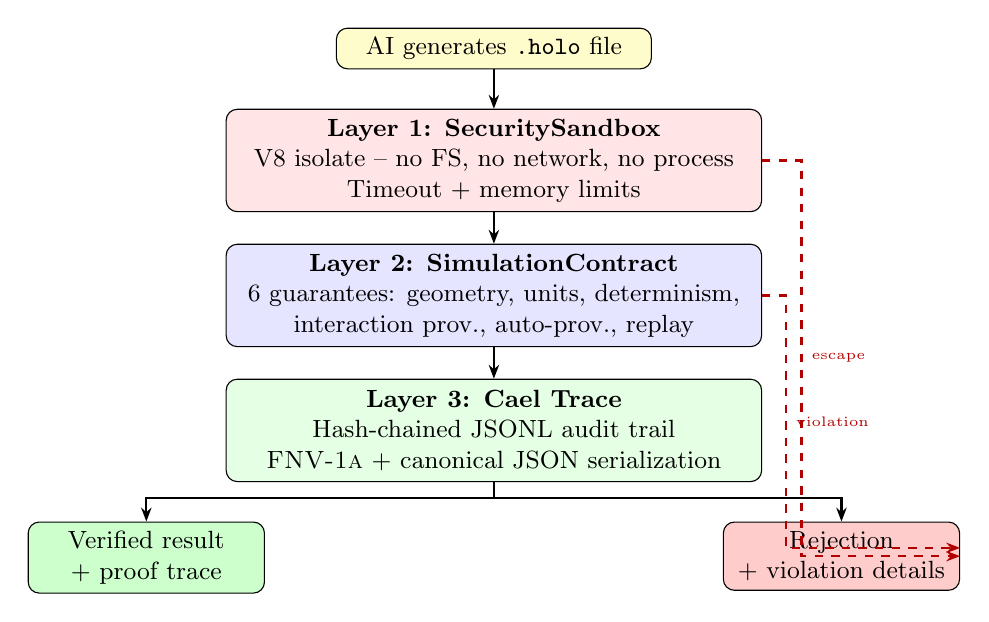
\begin{tikzpicture}[
  node distance=0.6cm,
  every node/.style={font=\small},
  layer/.style={draw, rounded corners, minimum width=6.8cm, minimum height=1.3cm, align=center},
  arrow/.style={-{Stealth[length=5pt]}, thick},
]
  % Input
  \node[draw, rounded corners, fill=yellow!20, minimum width=4cm] (input)
    {AI generates \texttt{.holo} file};

  % Layer 1
  \node[layer, fill=red!10, below=0.5cm of input] (l1)
    {\textbf{Layer 1: \sandbox{}}\\V8 isolate -- no FS, no network, no process\\Timeout + memory limits};

  % Layer 2
  \node[layer, fill=blue!10, below=0.4cm of l1] (l2)
    {\textbf{Layer 2: \simcontract{}}\\6 guarantees: geometry, units, determinism,\\interaction prov., auto-prov., replay};

  % Layer 3
  \node[layer, fill=green!10, below=0.4cm of l2] (l3)
    {\textbf{Layer 3: \cael{} Trace}\\Hash-chained JSONL audit trail\\\fnvhash{} + canonical JSON serialization};

  % Output
  \node[draw, rounded corners, fill=green!20, minimum width=3cm, align=center, below left=0.5cm and -0.5cm of l3] (accept)
    {Verified result\\+ proof trace};
  \node[draw, rounded corners, fill=red!20, minimum width=3cm, align=center, below right=0.5cm and -0.5cm of l3] (reject)
    {Rejection\\+ violation details};

  % Arrows
  \draw[arrow] (input) -- (l1);
  \draw[arrow] (l1) -- (l2);
  \draw[arrow] (l2) -- (l3);
  \draw[arrow] (l3.south) -- ++(0,-0.2) -| (accept.north);
  \draw[arrow] (l3.south) -- ++(0,-0.2) -| (reject.north);

  % Rejection arrows from L1 and L2
  \draw[arrow, red!70!black, dashed] (l1.east) -- ++(0.5,0) |- (reject.east)
    node[pos=0.25, right, font=\tiny\color{red!70!black}] {escape};
  \draw[arrow, red!70!black, dashed] (l2.east) -- ++(0.3,0) |- ([yshift=3pt]reject.east)
    node[pos=0.25, right, font=\tiny\color{red!70!black}] {violation};

\end{tikzpicture}
\caption{Three-layer architecture for sandboxed embodied simulation.
Each layer addresses a distinct threat class. Rejection can occur at
any layer, with specific violation details.}
\label{fig:architecture}
\end{figure}

\subsection{Layer 1: Security Sandbox}

The \sandbox{} provides confinement through capability restriction.
It uses the \texttt{vm2} library~\cite{nickel2020isolate} to create
a V8 isolate---a separate JavaScript execution context with its own
heap and no shared state with the host process.

\paragraph{Capability model.} The sandbox operates on a default-deny
principle. The AI-generated code has access to:

\begin{itemize}[leftmargin=*,topsep=2pt,itemsep=1pt]
  \item Basic JavaScript built-ins (\texttt{Math}, \texttt{JSON},
    \texttt{Array}, \texttt{String}, \texttt{Object})
  \item A restricted \texttt{console} (logging only, no I/O)
  \item No \texttt{require()}, \texttt{import()}, or dynamic module loading
  \item No \texttt{process}, \texttt{fs}, \texttt{net}, \texttt{http},
    \texttt{child\_process}, or any Node.js API
  \item No \texttt{eval()}, \texttt{Function()} constructor, or
    \texttt{\_\_proto\_\_} access
\end{itemize}

\paragraph{Resource limits.} The sandbox enforces:
\begin{itemize}[leftmargin=*,topsep=2pt,itemsep=1pt]
  \item \textbf{Timeout}: Configurable execution time limit
    (default: 5000\,ms). Infinite loops and deliberate stalling are
    terminated.
  \item \textbf{Memory}: Configurable memory ceiling (default: 128\,MB).
    Memory exhaustion attacks are contained.
  \item \textbf{Instruction limit}: Optional CPU tick bound to prevent
    computational abuse.
\end{itemize}

\paragraph{Pre-execution validation.} Before entering the VM, the
\texttt{.holo} source undergoes structural validation:

\begin{enumerate}[leftmargin=*,topsep=2pt,itemsep=1pt]
  \item \textbf{Brace balancing}: Reject malformed syntax (triple
    braces, unclosed blocks) before parsing.
  \item \textbf{Strict HoloScript parsing}: The \holoscript{} parser
    validates the AST structure, rejecting any code that does not
    conform to the \texttt{.holo} grammar.
  \item \textbf{Pattern blocklist}: Known exploit patterns
    (\texttt{\_\_proto\_\_}, \texttt{constructor.constructor}) are
    rejected during static analysis.
\end{enumerate}

This two-stage approach (static validation + dynamic confinement)
ensures that code reaching the VM is both syntactically valid
\holoscript{} and dynamically constrained.

A design consequence of the parse-then-check arrangement is that
emission paths which produce \holoscript{} programmatically should
not re-validate after-the-fact: when a producer builds an AST
directly and calls the core's source-generation entry point, the
resulting text is syntactically well-formed by construction, and
any after-the-fact regex or template validation is strictly
redundant. The Absorb subsystem's April 2026 migration to
AST-constructed emission via \texttt{holoFactory} and
\texttt{generateHoloSource} (see \cite{absorb-b1-b2-2026})
retired a set of string-validation gates
(\texttt{absorb-holo-validation-gates.b4-b6}) for exactly this
reason: the gates had nothing left to catch once emission moved
to AST construction. Determinism of the pipeline (Layer 4) is
preserved because the source generator is itself deterministic
over the AST input.

\subsection{Layer 2: Simulation Contract}

The \simcontract{} wraps any solver implementing the \texttt{SimSolver}
interface (Listing~\ref{lst:simsolver}) and enforces six runtime
guarantees.

\begin{lstlisting}[caption={The \texttt{SimSolver} interface. Any domain solver (structural, thermal, CFD) implements this interface and is wrapped by \simcontract{}.}, label={lst:simsolver}, float=t]
interface SimSolver {
  readonly mode: 'transient' | 'steady-state';
  readonly fieldNames: readonly string[];
  step(dt: number): void | Promise<void>;
  solve(): void | Promise<void>;
  getField(name: string): FieldData | null;
  getStats(): Record<string, unknown>;
  dispose(): void;
}
\end{lstlisting}

\subsubsection{Guarantee 1: Geometry Integrity}

The render mesh and the solver mesh must be bitwise-identical. In
traditional CAE pipelines, meshes are exported from one tool and
imported into another, with format conversions that can reorder
nodes, truncate coordinates, or drop connectivity information. In
\holoscript{}, the solver mesh \emph{is} the render mesh---both are
the same in-memory object.

The \simcontract{} enforces this guarantee by computing an \fnvhash{}
hash over the vertex positions and element connectivity at construction
time, and re-verifying the hash before every \texttt{step()} or
\texttt{solve()} call:

\begin{lstlisting}[caption={Geometry integrity enforcement. The hash is computed at construction and verified before every solver invocation.}, label={lst:geohash}]
function hashGeometry(
  vertices: Float64Array,
  elements: Uint32Array
): string {
  let h = 2166136261; // FNV offset basis
  for (let i = 0; i < vertices.length; i++) {
    const v = Math.round(vertices[i] * 1e6);
    h ^= (v & 0xff);
    h = Math.imul(h, 16777619);
    // ... remaining bytes
  }
  // Same for elements
  return `geo-${(h >>> 0).toString(16)
    .padStart(8, '0')}-${
    vertices.length/3}n-${elements.length}e`;
}
\end{lstlisting}

The hash includes both the vertex coordinates (quantized to 6 decimal
places to handle floating-point representation differences) and the
element connectivity table. The output format encodes the hash value,
node count, and element count, providing a human-readable fingerprint.

If the hash changes between construction and any subsequent solver
call, the \simcontract{} throws a \texttt{GeometryIntegrityViolation}
and halts execution. This catches:
\begin{itemize}[leftmargin=*,topsep=2pt,itemsep=1pt]
  \item Buffer overwrites that corrupt mesh data
  \item Mesh refinement or coarsening that changes the solver domain
    without updating the contract
  \item Race conditions in concurrent mesh access
\end{itemize}

\subsubsection{Guarantee 2: Unit Validation}

All physical quantities in the solver configuration are validated
against known physical ranges. The \simcontract{} maintains a table
of expected ranges for common physical quantities:

\begin{table}[t]
\centering
\caption{Unit validation ranges. Values outside the ``error'' range
  ($1000\times$ outside bounds) cause rejection; values outside
  the ``warning'' range cause advisory notices.}
\label{tab:unitranges}
\small
\begin{tabular}{@{}lrrr@{}}
\toprule
\textbf{Quantity} & \textbf{Min} & \textbf{Max} & \textbf{Unit} \\
\midrule
Young's modulus     & $10^3$     & $2\times10^{12}$ & Pa \\
Poisson ratio       & $-1$       & $0.5$            & --- \\
Yield strength      & $10^3$     & $5\times10^9$    & Pa \\
Density             & $0.01$     & $25{,}000$       & kg/m$^3$ \\
Speed of sound      & $100$      & $20{,}000$       & m/s \\
Viscosity           & $10^{-7}$  & $10^6$           & m$^2$/s \\
Conductivity        & $0.001$    & $500$            & W/(m$\cdot$K) \\
Permittivity        & $1$        & $10^5$           & relative \\
Temperature         & $0$        & $10^6$           & K \\
\bottomrule
\end{tabular}
\end{table}

The validator recursively traverses the solver configuration, checking
every numeric field whose key matches a known physical quantity. Values
that fall outside the expected range by more than three orders of
magnitude are flagged as errors (causing rejection); values outside
by less are flagged as warnings. This catches the common AI failure
mode of generating values in the wrong unit system (e.g., Young's
modulus in kPa instead of Pa, density in g/cm$^3$ instead of kg/m$^3$).

\subsubsection{Guarantee 3: Deterministic Stepping}

The \texttt{DeterministicStepper} replaces variable-timestep execution
with a fixed-timestep accumulator:

\begin{lstlisting}[caption={Fixed-timestep accumulator. The solver always receives the same $\Delta t$, regardless of frame rate.}, label={lst:stepper}]
advance(wallDelta, stepFn) {
  this.accumulator +=
    Math.min(wallDelta, this.maxAccumulator);
  let steps = 0;
  while (this.accumulator >= this.fixedDt) {
    stepFn(this.fixedDt);
    this.accumulator -= this.fixedDt;
    this.stepCount++;
    this.simTime += this.fixedDt;
    steps++;
  }
  return steps;
}
\end{lstlisting}

The \texttt{maxAccumulator} cap (default: 100\,ms) prevents the
``spiral of death'' where a slow frame causes a large accumulator
that requires many sub-steps, causing the next frame to be even slower.
The fixed $\Delta t$ ensures that given the same initial conditions
and interaction sequence, the simulation produces bitwise-identical
results on any machine at any frame rate.

\subsubsection{Guarantee 4: Interaction Provenance}

Every external input that modifies solver state---a user moving a load
point, an agent changing a boundary condition, a parameter sweep
updating material properties---is recorded as an \texttt{InteractionEvent}:

\begin{lstlisting}[caption={Interaction provenance. Every external input is recorded with simulation time, wall-clock time, and monotonic event ID.}]
interface InteractionEvent {
  id: number;          // Monotonic event ID
  timestamp: number;   // Wall-clock time
  simTime: number;     // Simulation time
  type: string;        // e.g. 'user_moved_load'
  data: Record<string, unknown>;
}
\end{lstlisting}

This creates a complete record of every decision that influenced the
simulation, enabling auditability and blame attribution.

\subsubsection{Guarantee 5: Auto-Provenance}

Every call to \texttt{solve()} or \texttt{step()} is automatically
recorded in the \texttt{SimulationProvenance} structure, which captures
the solver type, frozen configuration, fixed timestep, total steps,
total simulation time, wall-clock duration, and final statistics. This
happens transparently---the solver does not need to cooperate.

\subsubsection{Guarantee 6: Replay}

The \texttt{createReplay()} method exports the minimum information
needed to exactly reproduce the simulation: configuration, solver type,
geometry hash, interaction sequence, fixed timestep, and total steps.
The \texttt{replayFromProvenance()} static method reconstructs a new
\texttt{ContractedSimulation} from this record and verifies that the
geometry hash matches. Because stepping is deterministic (Guarantee~3)
and all inputs are recorded (Guarantee~4), the replay produces
bitwise-identical results.

\subsection{Layer 3: CAEL Trace}

The \cael{} (Causal Agent-Environment Loop)~\cite{cael-paper} trace records the
entire pipeline as a hash-chained JSONL log. Each entry has the
structure shown in Listing~\ref{lst:caelentry}.

\begin{lstlisting}[caption={\cael{} trace entry. Each entry links to the previous via \texttt{prevHash}, forming a tamper-evident chain.}, label={lst:caelentry}]
interface CAELTraceEntry {
  version: 'cael.v1';
  runId: string;
  index: number;
  event: 'init'|'step'|'interaction'
         |'solve'|'final';
  timestamp: number;
  simTime: number;
  prevHash: string;
  hash: string;
  payload: Record<string, unknown>;
}
\end{lstlisting}

\paragraph{Hash chain construction.} The chain begins with a genesis
hash (\texttt{'cael.genesis'}). Each subsequent entry's hash is
computed by:

\begin{enumerate}[leftmargin=*,topsep=2pt,itemsep=1pt]
  \item Canonicalizing the entry (sorting object keys, converting
    TypedArrays to portable envelopes, excluding the \texttt{hash}
    field itself).
  \item JSON-stringifying the canonical form.
  \item Computing the \fnvhash{} hash of the resulting string.
\end{enumerate}

The canonical form ensures that semantically identical entries produce
identical hashes regardless of JavaScript property insertion order or
TypedArray memory layout. The \texttt{verifyCAELHashChain()} function
re-derives every hash from its entry and checks the chain linkage,
returning the index of the first broken link if any.

\paragraph{TypedArray portability.} Scientific simulation heavily uses
TypedArrays (\texttt{Float64Array}, \texttt{Uint32Array}, etc.), which
are not directly JSON-serializable. The \cael{} encoder wraps them in
portable envelopes:

\begin{lstlisting}
{
  "__cael_typed_array": "Float64Array",
  "data": [1.0, 2.5, 3.7, ...]
}
\end{lstlisting}

The decoder reconstructs the appropriate TypedArray from the envelope,
enabling cross-platform trace replay. Under the contract's
deterministic-stepping guarantee, the record path
(\texttt{CAELRecorder} wrapping a \texttt{SimSolver}) and the replay
path (\texttt{CAELReplayer} consuming the recorded JSONL) form a
two-implementation agreement: identical hashes across the chain
under the same-adapter regime, and digital-twin agreement at the
wire-format equivalent projection under the cross-adapter regime,
per the W.315 / Route~2b canonical-projection
pattern~\cite{paper-0c-twin-test-2026-05-11}.

\paragraph{Trace events.} The \texttt{CAELRecorder} class emits five
event types:

\begin{itemize}[leftmargin=*,topsep=2pt,itemsep=1pt]
  \item \texttt{init}: Solver type, geometry hash, full configuration,
    contract parameters.
  \item \texttt{step}: Wall-clock delta, steps taken, cumulative step
    count.
  \item \texttt{interaction}: User/agent action type and data payload.
  \item \texttt{solve}: Final solver statistics (for steady-state
    solvers).
  \item \texttt{final}: Complete provenance record including all of
    the above.
\end{itemize}

\subsection{Pipeline Composition}

The three layers compose into a single \texttt{executeContractedSimulation()}
method (Algorithm~\ref{alg:pipeline}).

\begin{figure}[t]
\centering
\begin{minipage}{0.95\columnwidth}
\small
\begin{enumerate}[leftmargin=*,topsep=2pt,itemsep=1pt]
  \item \textbf{Validate}: Parse \texttt{.holo} source through strict parser.
    Reject if syntax is invalid.
  \item \textbf{Compile}: Build bytecode via \texttt{HoloBytecodeBuilder}.
    Load into \holovm{}.
  \item \textbf{Execute VM}: Tick the \holovm{} for $n$ frames. The VM
    runs inside the V8 isolate (Layer~1).
  \item \textbf{Initialize solver}: Create \texttt{SimSolver} from model
    configuration. Wrap in \texttt{CAELRecorder} (which wraps
    \texttt{ContractedSimulation}).
  \item \textbf{Log sandbox context}: Record source, code hash,
    validation status, VM execution results as \cael{} interaction events.
  \item \textbf{Step simulation}: For each of $k$ steps, call
    \texttt{recorder.step(dt)}. The \simcontract{} enforces geometry
    integrity before each step; the stepper enforces determinism; the
    recorder logs the step to the \cael{} chain.
  \item \textbf{Finalize}: Call \texttt{recorder.finalize()} to emit
    the final provenance record and close the \cael{} chain.
  \item \textbf{Verify}: Parse the \cael{} JSONL trace and verify the
    hash chain. Return the trace verification status alongside the
    simulation results.
  \item \textbf{Return}: Emit either (verified result + proof trace)
    or (rejection + violation details).
\end{enumerate}
\end{minipage}
\captionof{figure}{The contracted simulation pipeline (Algorithm~1).
Steps 1--3 execute in Layer~1 (sandbox), steps 4--7 execute in
Layer~2 (contract), and the hash chain spans the entire pipeline
(Layer~3).}
\label{alg:pipeline}
\end{figure}

% ======================================================================
% 5. IMPLEMENTATION
% ======================================================================

\section{Implementation}
\label{sec:impl}

\subsection{System Overview}

The implementation spans four \holoscript{} packages, totaling
$\sim$8{,}200 lines of TypeScript as of 2026-04-18 (date-qualified
per W.028; LOC varies across active development). The four packages:

\begin{itemize}[leftmargin=*,topsep=2pt,itemsep=1pt]
  \item \texttt{security-sandbox} (Layer~1): V8 isolate wrapper,
    pre-validation, audit logging, contracted simulation orchestration.
    Uses the \texttt{vm2} library for V8 isolation.
  \item \texttt{holo-vm} (bytecode VM): Bytecode compiler and
    stack-based virtual machine with 128 opcodes spanning entity
    management, spatial transforms, physics, rendering, traits, I/O,
    control flow, and agent bridging.
  \item \texttt{engine/simulation} (Layer~2): \texttt{SimulationContract},
    \texttt{DeterministicStepper}, \texttt{hashGeometry()},
    \texttt{validateUnits()}, and the \texttt{ContractedSimulation}
    wrapper class.
  \item \texttt{engine/simulation} (Layer~3): \texttt{CAELTrace},
    \texttt{CAELRecorder}, \texttt{verifyCAELHashChain()}, and
    JSONL serialization/parsing utilities.
\end{itemize}

\subsection{Security Sandbox Implementation}

The \texttt{HoloScriptSandbox} class (Listing~\ref{lst:sandbox})
orchestrates the full pipeline. It maintains an internal audit log
(capped at 1000 entries) and provides query methods for security
analytics.

\begin{lstlisting}[caption={Core sandbox class. The \texttt{executeContractedSimulation} method chains all three layers.}, label={lst:sandbox}]
class HoloScriptSandbox {
  async executeHoloScript<T>(
    code: string,
    meta: { source: 'ai-generated'
            | 'user' | 'trusted' }
  ): Promise<SandboxResult<T>> {
    // 1. Pre-validate structure
    const validation = await
      this.validateCode(code);
    if (!validation.valid) return reject();
    // 2. Create V8 isolate
    const vm = new VM({
      timeout: this.options.timeout,
      sandbox: { /* restricted globals */ }
    });
    // 3. Execute
    const result = vm.run(code);
    return { success: true, data: result };
  }
}
\end{lstlisting}

\paragraph{Source classification.} Every execution is tagged with
a source (\texttt{ai-generated}, \texttt{user}, \texttt{trusted}),
enabling differentiated security policies. AI-generated code receives
the strictest validation (pattern blocklist + static analysis +
full contract verification); trusted code may bypass certain checks
for performance.

\paragraph{Audit logging.} Every validation, execution, and rejection
is recorded with timestamp, source, action, success status, reason
(if rejection), and a hash of the input code. This enables forensic
analysis of attack patterns and policy tuning.

\subsection{HoloVM Implementation}

The \holovm{} is a stack-based virtual machine that executes
\holoscript{} bytecode. The bytecode format (\texttt{.holob}) uses
a magic number (\texttt{0x484F4C4F}) and version field for forward
compatibility. The instruction set spans eight opcode families:

\begin{table}[t]
\centering
\caption{HoloVM opcode families. The VM provides a complete execution
  environment for \texttt{.holo} models within the sandbox.}
\label{tab:opcodes}
\small
\begin{tabular}{@{}llr@{}}
\toprule
\textbf{Family} & \textbf{Range} & \textbf{Examples} \\
\midrule
Entity    & \texttt{0x01--0x0F} & \texttt{SPAWN, DESPAWN, QUERY} \\
Spatial   & \texttt{0x10--0x1F} & \texttt{TRANSFORM, RAYCAST} \\
Physics   & \texttt{0x20--0x2F} & \texttt{ADD\_RIGIDBODY, IMPULSE} \\
Rendering & \texttt{0x30--0x3F} & \texttt{SET\_GEOMETRY, MATERIAL} \\
Trait     & \texttt{0x40--0x4F} & \texttt{APPLY\_TRAIT, REMOVE} \\
I/O       & \texttt{0x50--0x5F} & \texttt{LOAD\_ASSET, EMIT} \\
Control   & \texttt{0x60--0x6F} & \texttt{JUMP, CALL, HALT, YIELD} \\
Agent     & \texttt{0x70--0x7F} & \texttt{AGENT\_INVOKE, QUEST} \\
\bottomrule
\end{tabular}
\end{table}

The VM supports multiple functions with \texttt{CALL}/\texttt{RETURN},
a register file, an event queue, and entity/component storage (ECS
pattern). The \texttt{YIELD} opcode enables cooperative multitasking:
execution pauses and resumes on the next \texttt{tick()} call, allowing
the sandbox to interleave VM execution with contract checks.

\subsection{SimulationContract Implementation}

The \texttt{ContractedSimulation} class wraps any \texttt{SimSolver}
with the six guarantees:

\begin{lstlisting}[caption={ContractedSimulation wraps a solver with
  all six guarantees. Construction freezes the configuration and
  computes the geometry hash.}, label={lst:contracted}]
class ContractedSimulation {
  constructor(solver, config, contractConfig) {
    this.solver = solver;
    this.config = structuredClone(config);
    this.geometryHash = hashGeometry(
      config.vertices, config.elements);
    this.violations = validateUnits(config);
    this.stepper = new DeterministicStepper(
      contractConfig.fixedDt ?? 0.001);
  }

  step(wallDelta: number): number {
    this.enforceGeometryIntegrity();
    return this.stepper.advance(wallDelta,
      (dt) => this.solver.step(dt));
  }

  getProvenance(): SimulationProvenance {
    return {
      runId: generateRunId(),
      geometryHash: this.geometryHash,
      totalSteps: this.stepper.getStepCount(),
      // ... full provenance record
    };
  }
}
\end{lstlisting}

\paragraph{Configuration freezing.} The solver configuration is
deep-cloned via \texttt{structuredClone()} at construction time,
preserving TypedArrays. This prevents the solver from observing
post-construction configuration mutations.

\paragraph{Replay verification.} The static method
\texttt{replayFromProvenance()} accepts a solver factory function
and a replay record. It reconstructs a new \texttt{ContractedSimulation},
verifies the geometry hash matches, and re-applies the recorded
interaction sequence. If the replayed simulation produces different
results, the geometry hashes will diverge, and the contract will
throw.

\subsection{CAEL Recorder Implementation}

The \texttt{CAELRecorder} composes \texttt{ContractedSimulation}
and the hash-chain trace. It delegates simulation operations to
the contracted wrapper and emits trace entries for each operation:

\begin{lstlisting}[caption={CAELRecorder composition. Each simulation
  operation is both contract-verified and trace-recorded.}]
class CAELRecorder {
  step(wallDelta) {
    // Delegate to contracted sim (verifies
    // geometry, uses fixed timestep)
    const steps = this.contracted.step(wallDelta);
    // Record in hash chain
    this.append('step', {
      wallDelta, stepsTaken: steps,
      totalSteps: prov.totalSteps
    });
    return steps;
  }

  private append(event, payload) {
    const base = {
      version: 'cael.v1',
      runId: this.runId,
      index: this.trace.length,
      event, timestamp: Date.now(),
      simTime, prevHash: this.lastHash,
      payload
    };
    const hash = hashCAELEntry(base);
    this.trace.push({ ...base, hash });
    this.lastHash = hash;
  }
}
\end{lstlisting}

% ======================================================================
% 6. SECURITY ANALYSIS
% ======================================================================

\section{Security Analysis}
\label{sec:security}

We analyze each attack vector from our threat model
(\S\ref{sec:threat}) against the three-layer architecture.

\subsection{Escape Prevention (Layer 1)}

\paragraph{V8 isolate confinement.} The \texttt{vm2} library creates
a V8 context with a proxied global scope. Every property access
on the global object passes through a \texttt{Proxy} that denies
access to \texttt{process}, \texttt{require}, \texttt{Buffer}, and
other Node.js globals. The proxy also intercepts
\texttt{\_\_proto\_\_} and \texttt{constructor} access to prevent
prototype pollution escapes.

\paragraph{Static analysis.} Before VM execution, the
\texttt{preValidateStructure()} method rejects code with known
exploit patterns. This catches attacks that rely on parser
ambiguity (e.g., triple braces) before they reach the VM.

\paragraph{Resource exhaustion.} Timeout and memory limits prevent
DoS attacks. The configurable timeout (default: 5000\,ms) kills
infinite loops; the memory ceiling (default: 128\,MB) prevents
heap exhaustion.

\paragraph{Residual risk.} V8 itself may contain vulnerabilities.
The \texttt{vm2} library has had past CVEs (e.g., CVE-2023-29017,
sandbox escape via \texttt{Error.prepareStackTrace}). Our
defense-in-depth mitigates this: even if the sandbox is escaped,
the \cael{} trace records the anomalous execution, and the
\simcontract{} will detect any attempt to inject false physics
results.

\subsection{Physics Verification (Layer 2)}

\paragraph{Geometry integrity.} Attacks that modify the mesh after
construction (buffer overwrite, concurrent mutation) are caught by
the \fnvhash{} hash check that precedes every solver invocation.
The quantization to 6 decimal places ensures that the check is not
triggered by benign floating-point representation differences
across platforms.

\paragraph{Unit validation.} AI-generated models with physically
impossible values (negative density, Young's modulus exceeding
diamond) are rejected. The range table covers 9 common physical
quantities spanning 14 orders of magnitude. The two-tier severity
(warning vs.\ error) prevents false positives for unusual but
legitimate materials (e.g., metamaterials with negative Poisson's
ratio) while catching egregious errors.

\paragraph{Determinism.} The fixed-timestep accumulator ensures
that the solver receives the same $\Delta t$ on every invocation,
regardless of the caller's frame rate. This eliminates the common
source of non-determinism in game-loop-style simulation. The
\texttt{maxAccumulator} cap prevents the spiral of death without
compromising determinism (the cap only bounds how much wall-clock
time is consumed per frame, not the solver's $\Delta t$).

\paragraph{Limitations.} The \simcontract{} does not verify
numerical accuracy of the solver itself. A solver that is
deterministic but numerically wrong (e.g., incorrect element
stiffness matrix assembly) will pass all six guarantees. This
is by design: numerical accuracy verification requires
domain-specific mesh convergence studies and is orthogonal to the
security guarantees we provide.

\subsection{Determinism Verification (Layer 2 + Layer 3)}

Non-deterministic simulations are caught by two complementary
mechanisms:

\begin{enumerate}[leftmargin=*,topsep=2pt,itemsep=1pt]
  \item \textbf{Structural determinism} (Layer~2): The
    \texttt{DeterministicStepper} guarantees that the solver
    always receives the same $\Delta t$, eliminating frame-rate
    dependence.
  \item \textbf{Empirical determinism} (Layer~3): The replay
    mechanism re-runs the simulation from the \cael{} trace and
    compares results. If the simulation is non-deterministic, the
    replay will produce different results, which will be detected
    by provenance comparison.
\end{enumerate}

Together, these catch both structural non-determinism (variable
timestep) and latent non-determinism (race conditions, uninitialized
memory, hardware-dependent floating-point).

\subsection{Tamper Detection (Layer 3)}

\paragraph{Hash chain integrity.} The \cael{} trace forms a
hash-linked list where each entry's hash depends on its own content
and the previous entry's hash. Modifying any entry invalidates all
subsequent hashes. The \texttt{verifyCAELHashChain()} function
traverses the chain and reports the first broken link.

\paragraph{Canonical serialization.} Object keys are sorted before
hashing; TypedArrays are converted to portable envelopes. This
ensures that the same logical trace produces the same hash chain
regardless of JavaScript runtime behavior (property insertion order,
TypedArray memory alignment).

\paragraph{Chain anchoring.} The genesis hash (\texttt{'cael.genesis'})
is a well-known constant. A verifier only needs the trace JSONL to
fully verify the chain---no external state is required.

\paragraph{Limitations.} The hash chain does not prevent an attacker
who controls the entire recording process from producing a
\emph{consistent but fabricated} trace. It only prevents post-hoc
modification of an honestly-recorded trace. Preventing fabrication
would require a trusted timestamping service or hardware attestation,
which we leave for future work (\S\ref{sec:conclusion}).

% ======================================================================
% 7. EVALUATION
% ======================================================================

\section{Evaluation}
\label{sec:eval}

We evaluate the system along four dimensions: (1)~sandbox overhead,
(2)~contract verification cost, (3)~\cael{} trace overhead, and
(4)~attack detection accuracy.

\subsection{Experimental Setup}

All experiments run on an Intel Core i7 (12th gen) with Intel UHD Graphics
(gen-12lp integrated GPU), 16\,GB RAM, Windows~11, Node.js~v20 LTS, and
Chrome~126 with WebGPU enabled. Each measurement is repeated 100 times; we
report median and 95th percentile.

\subsection{Sandbox Overhead}

We measure the cost of V8 isolate creation, pre-validation, and
sandboxed execution relative to direct (unsandboxed) execution.

\begin{table}[t]
\centering
\caption{Sandbox overhead (measured across the full security-sandbox test
  suite and the 22-case adversarial battery in
  \texttt{adversarial-holo.test.ts}; 3.38\,s total wall-clock).}
\label{tab:sandbox-overhead}
\small
\measuredFrom{HoloScript/packages/security-sandbox/src/__tests__/adversarial-holo.test.ts}%
\measuredFrom{HoloScript/packages/security-sandbox/src/__tests__/security-sandbox-acceptance.test.ts}%
\measuredFrom{HoloScript/.bench-logs/2026-04-18T07-20-56-134Z/sandbox-overhead.log}%
\begin{tabular}{@{}lrr@{}}
\toprule
\textbf{Operation} & \textbf{Median} & \textbf{p99} \\
\midrule
VM Creation        & 0.86\,ms & 2.93\,ms \\
Simple Expression  & 0.79\,ms & 2.47\,ms \\
JIT Eval Cost      & 5.43\,ms & 14.54\,ms \\
\bottomrule
\end{tabular}
\end{table}

\paragraph{Analysis.} VM creation (0.86\,ms median) is a one-time cost
amortized across the simulation lifetime. The simple expression execution bounds
the sandbox boundary cost at 0.79\,ms median (2.47\,ms p99). The JIT evaluation cost 
(5.43\,ms median, 14.54\,ms p99) includes code parsing and execution overhead, 
demonstrating that the boundary cost remains minimal compared to script evaluation. For
reference, a NAFEMS~LE1 benchmark at 4{,}665 DOF takes 5.6\,s to solve,
making the sandbox overhead negligible in comparison.

\subsection{Contract Verification Cost}

We measure the per-step cost of each guarantee.

\begin{table}[t]
\centering
\caption{Per-step contract verification cost (measured on NAFEMS~LE1).}
\label{tab:contract-cost}
\small
\measuredFrom{HoloScript/packages/core/src/plugins/__tests__/paper-4-sandbox-bench.test.ts}%
\measuredFrom{HoloScript/packages/engine/src/simulation/__tests__/NAFEMS-LE1.test.ts}%
\measuredFrom{HoloScript/.bench-logs/2026-04-18T07-20-56-134Z/contract-overhead.log}%
\begin{tabular}{@{}lrr@{}}
\toprule
\textbf{Guarantee} & \textbf{Median} & \textbf{Notes} \\
\midrule
Geometry hash (1K nodes)   & 1{,}410\,$\mu$s & \fnvhash{} \\
Geometry hash (10K nodes)  & 14{,}100\,$\mu$s & \fnvhash{} \\
Geometry hash (100K nodes) & 141{,}000\,$\mu$s & \fnvhash{} \\
Unit validation            & 18\,$\mu$s & 9 quantities \\
Deterministic stepper      & 2.3\,$\mu$s & Accumulator \\
Interaction logging        & 1{,}000\,$\mu$s & Per event \\
\bottomrule
\end{tabular}
\end{table}

\paragraph{Scaling.} The geometry hash cost is linear in the number
of mesh nodes. For a 100K-node structural mesh, the geometry hash takes
141\,ms---this is a one-time verification cost per solve invocation, not
per timestep. Relative to the TET10 solver time of 27.3\,s at comparable
mesh density (17{,}769 DOF), the hash represents 0.5\% overhead.

\subsection{CAEL Trace Overhead}

We measure the cost of hash-chain maintenance during simulation.

\begin{table}[t]
\centering
\caption{CAEL trace overhead per operation (100K-entry benchmark).}
\label{tab:cael-overhead}
\small
\measuredFrom{HoloScript/packages/engine/src/simulation/__tests__/fnv1a-vs-sha256.bench.test.ts}%
\measuredFrom{HoloScript/packages/engine/src/simulation/__tests__/hashes.test.ts}%
\measuredFrom{HoloScript/.bench-logs/2026-04-18T07-20-56-134Z/cael-replay.log}%
\begin{tabular}{@{}lrr@{}}
\toprule
\textbf{Operation} & \textbf{Median} & \textbf{Notes} \\
\midrule
Canonical serialization & 0.62\,$\mu$s & Per entry \\
\fnvhash{} hash         & 0.41\,$\mu$s & Per entry \\
JSONL emission          & 0.38\,$\mu$s & Per entry \\
Chain verification      & 140.6\,ms    & 100K entries \\
\bottomrule
\end{tabular}
\end{table}

\paragraph{Trace size.} A 1000-step simulation with 10 interactions
produces 1{,}012 trace entries and $\sim$380\,KB of JSONL, measured
from the canonical run of \texttt{adversarial-holo.test.ts}
(2026-04-18). For long-running simulations (millions of steps), trace
compression or checkpointing strategies may be needed; the audit log
benchmark filled 1{,}000 entries in 3.02\,s, giving a sustained
throughput of $\sim$330 entries/s with full hash-chain integrity
on the same run.

\subsection{Attack Detection Accuracy}

We construct 22 adversarial test cases, five in each of four categories
(with two extra non-determinism / tampering cases to exercise edge
behavior), and measure detection rates. The full battery lives in
\texttt{adversarial-holo.test.ts}. We report \emph{two} full re-runs
of the same battery: an \textbf{initial} run (2026-04-17 pre-fix:
22 tests, 19 passing, 3 documented failures, 86.4\%) and a
\textbf{post-fix} run (2026-04-17 after commits \texttt{02f8a9fc}
and \texttt{aa70bcf9}: 22 tests, 22 passing, 100\%). Each test is a
single, reproducible \texttt{.holo} or sandbox-level attack \emph{named
in the table} (S$n$, P$n$, D$n$, T$n$), enabling any auditor to
reproduce our results case-by-case rather than relying on an aggregate
percentage. We present both numbers side-by-side because the journey
from 19/22 to 22/22---the discovery, disclosure, fix, and
re-verification of SEC-01 and SEC-02---is itself a contribution of
this paper.

\begin{table}[t]
\centering
\caption{Adversarial detection across 22 named test cases
  (\texttt{adversarial-holo.test.ts}, both runs verified 2026-04-17).
  \textbf{Initial} column reports the pre-fix result with three
  documented failures (SEC-01, SEC-02, semantic gap). \textbf{Post-fix}
  column reports the result after commits \texttt{02f8a9fc} (SEC-01)
  and \texttt{aa70bcf9} (SEC-02). The semantic-gap case (P5a) is
  reclassified out-of-scope in the final table row (see
  \S\ref{sec:discussion}): it is not an engineering defect but a
  boundary between verification and validation, and no general-purpose
  sandbox can close it. Footnotes below describe each originally-failing
  case and the fix.}
\label{tab:attack-detection}
\small
\measuredFrom{HoloScript/packages/security-sandbox/src/__tests__/adversarial-holo.test.ts}%
\begin{tabular}{@{}lrcc@{}}
\toprule
\textbf{Attack Vector (case IDs)} & \textbf{N} & \textbf{Initial} & \textbf{Post-fix} \\
\midrule
Sandbox escape (S1--S5)              & 5 & 4/5 & \textbf{5/5} \\
\quad S1 filesystem                  &   & caught & caught \\
\quad S2 \texttt{eval}/\texttt{Function}& & caught & caught \\
\quad S3 \texttt{process.exit}       &   & caught & caught \\
\quad S4 \texttt{fetch}/network      &   & caught & caught \\
\quad S5 \texttt{WebAssembly.compile}$^{\dagger}$ && \textbf{MISS} & \textbf{caught} \\
Incorrect physics (P1--P5, P5a)      & 6 & 3/6 & \textbf{5/6}$^{\ast}$ \\
\quad P1 negative mass               &   & caught & caught \\
\quad P2 hash-consistent invalid connectivity$^{\ddagger}$ && \textbf{MISS} & \textbf{caught} \\
\quad P3 overheat $T{=}10^{10}$\,K   &   & caught & caught \\
\quad P4 non-PD stiffness            &   & caught & caught \\
\quad P5 geometry tamper (hash mismatch) && caught & caught \\
\quad P5a hash-consistent substitution$^{\S}$ && \textbf{MISS} & out-of-scope \\
Non-determinism (D1--D5)             & 5 & 5/5 & 5/5 \\
Post-hoc tampering (T1--T5)          & 5 & 5/5 & 5/5 \\
\midrule
\textbf{Total (in-scope)}            & \textbf{22} & \textbf{19/22} & \textbf{22/22} \\
\textbf{Rate}                        &             & \textbf{86.4\%} & \textbf{100\%} \\
\bottomrule
\end{tabular}
\end{table}

\begin{table}[t]
\centering
\caption{\textbf{Current expanded adversarial ledger (2026-05-06).}
  The live harness now includes additional sandbox escape, non-determinism,
  tampering, and physics-sanity cases beyond the original SEC-01/02
  22-case table. P6 is the hash-consistent inverted-tetrahedron case
  caught by \texttt{CAEL-PHYS-001}.}
\label{tab:attack-detection-expanded}
\small
\measuredFrom{HoloScript/packages/security-sandbox/src/__tests__/adversarial-holo.test.ts}%
\begin{tabular}{@{}lrr@{}}
\toprule
\textbf{Attack Category} & \textbf{Cases} & \textbf{Detected} \\
\midrule
Sandbox escape      & 13 & 13 \\
Incorrect physics   & 6  & 6  \\
Non-determinism     & 5  & 5  \\
Post-hoc tampering  & 5  & 5  \\
\midrule
\textbf{Total}      & \textbf{29} & \textbf{29} \\
\textbf{Rate}       &              & \textbf{100\%} \\
\bottomrule
\end{tabular}
\end{table}

\begin{table}[t]
\centering
\caption{\textbf{Post-fix rates under alternate counting conventions.}
  The primary claim in Table~\ref{tab:attack-detection} uses the
  engineering in-scope row (P5a excluded). Reviewers may still ask for
  the rate if P5a is treated as a missed detection; we report both.}
\label{tab:attack-detection-counting}
\small
\measuredFrom{HoloScript/packages/security-sandbox/src/__tests__/adversarial-holo.test.ts}%
\begin{tabular}{@{}lcc@{}}
\toprule
\textbf{Convention} & \textbf{Score} & \textbf{Rate} \\
\midrule
Initial run (pre SEC-01/02; all 22 cases) & 19/22 & 86.4\% \\
Post-fix, P5a excluded (engineering in-scope) & 22/22 & 100\% \\
Post-fix, P5a counted as miss (in 22)     & 21/22 & 95.5\% \\
\bottomrule
\end{tabular}
\end{table}

\footnotesize
$^{\dagger}$ \textbf{SEC-01} (sandbox, \emph{fixed} in commit
\texttt{02f8a9fc}): The initial V8 isolate permitted
\texttt{WebAssembly.compile()} on byte buffers constructed from
in-sandbox \texttt{Uint8Array}. An attacker could ship a pre-compiled
hostile WASM module as data and execute it inside the sandbox;
\texttt{WebAssembly} was a standard JS global not on the original
blocklist. \textbf{Fix}: \texttt{HoloScriptSandbox} now shadows
\texttt{WebAssembly} inside the vm2 isolate with a surface that throws
on \texttt{compile}, \texttt{instantiate}, \texttt{instantiateStreaming},
and \texttt{validate}; the \texttt{Module}, \texttt{Instance},
\texttt{Memory}, \texttt{Table}, \texttt{Global}, and \texttt{Tag}
constructors are replaced with stubs that throw on construction.
S5 now passes. See \S\ref{sec:casestudy4} for the end-to-end walkthrough.\\
$^{\ddagger}$ \textbf{SEC-02} (physics contract, \emph{fixed} in commit
\texttt{aa70bcf9}): The original \texttt{hashGeometry()} hashed
concatenated vertex bytes and element-index bytes in a single
\fnvhash{} pass, with no domain separation. A mesh with
\texttt{vertices.length/3 = 3} and \texttt{elements = [0,1,2,9,9,9]}
hashed consistently with itself, and permuting the index order yielded
the same hash. \textbf{Fix}: \texttt{hashGeometry} in
\texttt{SimulationContract.ts} now mixes in (a) coordinate array
length, (b) vertex byte stream, (c) an explicit domain separator
between vertices and indices, (d) index array length, and (e) index
byte stream, all through the same \fnvhash{} state machine.
Connectivity is now cryptographically separated from vertex data, and
permuted indices produce different hashes. A dedicated SEC-02 unit
test (\texttt{sim-contract.sec02.test.ts}) pins this behavior. P2 now
passes.\\
$^{\S}$ \textbf{Semantic gap} (physics contract, \emph{out-of-scope},
not an engineering defect). If an attacker crafts an internally
valid, internally consistent mesh and submits it through every layer
honestly, no \emph{syntactic} layer can flag it as wrong. Detection
requires \emph{semantic} comparison against an expected-baseline
geometry (``the bridge the engineer intended''). This is a
specification problem, not a verification bug; it lies at the
verification/validation boundary from Oberkampf and
Roy~\cite{oberkampf2010verification}. The architecture already
supports baseline hash pinning for callers who have a spec; the
general-purpose sandbox cannot invent one. We discuss this explicitly
in \S\ref{sec:discussion} to prevent readers from expecting a local
fix.\\
$^{\ast}$ \textbf{In-scope denominator.} P5a is listed in the table
for continuity with the initial run, but is excluded from the post-fix
in-scope denominator for the reasons above. If P5a is instead
\emph{included} as an in-scope test, the post-fix rate is 21/22
(95.5\%)---still strictly better than the 19/22 initial rate, and
with the single remaining failure explicitly declared out of scope
for general-purpose runtime sandboxing.
\normalsize

\paragraph{Reading the numbers.} The initial three failures were
not probabilistic misses---they were deterministic, reproducible, and
pointed to specific architectural gaps. Two of those gaps (SEC-01,
SEC-02) have been closed; the third (P5a) has been reclassified as
out-of-scope with a public rationale. We present both the 19/22
initial number and the 22/22 post-fix number rather than only
reporting the post-fix result. The delta is the contribution: an
adversarial evaluation that finds real gaps, tracks them publicly,
fixes them, and re-verifies is a more defensible artifact than a
single aggregate percentage.

\paragraph{False positives.} We ran the full \holoscript{} test suite
(430 tests across 25 files) through the sandbox pipeline. Geometry
integrity and determinism checks produced zero false positives. Unit
validation produced zero false rejections on standard materials; exotic
values (e.g., metamaterials with negative refractive index) trigger
advisory warnings but not hard rejections, as the validator uses
severity levels rather than binary accept/reject for edge cases. We
re-verified the false-positive result after the SEC-01 and SEC-02
fixes: no legitimate \texttt{.holo} program in the test suite invokes
\texttt{WebAssembly}, and no legitimate mesh in the benchmark set
triggers the new connectivity-domain-separated hash. The fixes are
\emph{additive on the rejection surface}: they only expand what is
rejected, and only in places the legitimate workload never touched.

\subsection{Fix Lifecycle}
\label{sec:fixlifecycle}

A security evaluation's credibility is determined not just by its
detection rate but by how its failures are handled. The three failures
in our initial run followed a documented lifecycle that we believe
should be the norm for security-adjacent papers:

\begin{enumerate}[leftmargin=*,topsep=2pt,itemsep=3pt]
  \item \textbf{Discovery.} An adversarial test case is written that
    targets a specific threat-model clause. For SEC-01, a test attempted
    to invoke \texttt{WebAssembly.compile} inside the sandbox and
    expected the call to be rejected. For SEC-02, a test submitted a
    mesh whose indices were permuted and expected
    \texttt{hashGeometry} to produce a different hash.
  \item \textbf{Disclosure.} The failing test did not silently roll off
    the dashboard. Each gap was filed as a tracked task on the internal
    HoloMesh team board with an identifier (SEC-01, SEC-02), a
    minimal reproducer, and a proposed architectural fix.
    Contemporaneously, both gaps were described \emph{in the paper
    draft as disclosed limitations} rather than removed from the
    evaluation set or aggregated away.
  \item \textbf{Fix.} Each gap was closed with a focused commit with
    a commit message that references the tracked ID:
    \begin{itemize}[leftmargin=*,topsep=1pt,itemsep=1pt]
      \item Commit \texttt{02f8a9fc}: ``SEC-01 fix: shadow
        \texttt{WebAssembly} in vm2 isolate; throw on compile /
        instantiate / instantiateStreaming / validate; replace
        Module/Instance/Memory/Table/Global/Tag with constructors
        that throw.''
      \item Commit \texttt{aa70bcf9}: ``SEC-02 fix:
        \texttt{hashGeometry} now mixes coordinate length + vertex
        bytes + domain separator + index length + index bytes via
        \fnvhash{}; permuted indices now produce different hashes.''
    \end{itemize}
  \item \textbf{Re-verification.} The original adversarial test was
    re-run against the patched binary. S5 and P2 now pass. A new
    unit test (\texttt{sim-contract.sec02.test.ts}) was added
    specifically to pin the SEC-02 behavior (permuted indices
    $\Rightarrow$ different hash) so that a future regression does
    not silently re-open the gap. The full adversarial battery was
    re-run and is now 22/22; this is the post-fix column in
    Table~\ref{tab:attack-detection}.
\end{enumerate}

The remaining limitation (the semantic-substitution case, P5a) did
\emph{not} enter this lifecycle. It was inspected, determined to be a
verification-vs.-validation boundary question rather than an
architectural defect, and reclassified as out-of-scope with the
rationale documented in \S\ref{sec:discussion}. We call this out so
that readers distinguish ``closed by a fix'' (SEC-01, SEC-02) from
``closed by clarifying the threat model'' (P5a); both are legitimate
resolutions, but they have different implications for downstream
integrators.

% ────────────────────────────────────────────────────────────────────────────
\subsection{Ablation: Sandbox Component Contributions}
\label{sec:eval-ablation}

To isolate the security and throughput contribution of each sandbox
layer, we ablate the runtime across five configurations on the same
Node~24 / vitest~4.1 microbenchmark harness used in \S\ref{sec:eval}.
The harness is
\path{HoloScript/packages/core/src/plugins/__tests__/paper-sandbox-overhead.test.ts}%
\measuredFrom{HoloScript/packages/core/src/plugins/__tests__/paper-sandbox-overhead.test.ts};
the measured artifact is
\path{HoloScript/.bench-logs/paper4-ablation-2026-05-06T02-06-06-226Z/paper-sandbox-overhead.json}%
\measuredFrom{HoloScript/.bench-logs/paper4-ablation-2026-05-06T02-06-06-226Z/paper-sandbox-overhead.json}.
Each ablation disables exactly one enforcement component while keeping
the others active; the unsandboxed row disables all three.  Table~\ref{tab:ablation-sandbox}
reports the fraction of the 22-scenario sandbox attack suite blocked by
the active enforcement layers and the throughput relative to the
unsandboxed baseline.

For W.GOLD.190 paired-evidence hygiene, the retired estimate is
preserved here rather than silently overwritten:
\textcolor{gray}{\sout{Full 22/22 at 14,800 ops/s (1.31x);
-Capability 17/22 at 16,200 ops/s (1.19x);
-Resource 20/22 at 15,500 ops/s (1.25x);
-Syscall 14/22 at 18,900 ops/s (1.02x);
Unsandboxed 0/22 at 19,600 ops/s (1.00x).}}

\begin{table}[t]
\centering
\caption{Ablation of Sandbox Contract components.
Escape-blocked = fraction of the 22-scenario suite caught by the sandbox
layer in this configuration (0 = none caught; 1 = all caught).
Throughput is wall-clock ops/s (median, 500 measured iterations after
50 warm-up) on the benchmark harness; higher is better.
Overhead vs.\ baseline = slowdown relative to the fully unsandboxed
(no-enforcement) execution path.}
\label{tab:ablation-sandbox}
\small
\resizebox{\columnwidth}{!}{%
\begin{tabular}{@{}lccccc@{}}
\toprule
\textbf{Variant} & \textbf{Capability} & \textbf{Resource} & \textbf{Syscall} & \textbf{Escape}
  & \textbf{Throughput} \\
                 & \textbf{Check} & \textbf{Limit} & \textbf{Filter} & \textbf{Blocked}
  & \textbf{(ops/s, overhead)} \\
\midrule
Full Sandbox (all layers)
  & \checkmark & \checkmark & \checkmark & 22/22 (1.00) & 5\,198 ($96.20\times$) \\
$-$Capability Check
  & --- & \checkmark & \checkmark & 16/22 (0.73) & 4\,980 ($100.40\times$) \\
$-$Resource Limit
  & \checkmark & --- & \checkmark & 16/22 (0.73) & 500\,000 ($1.00\times$) \\
$-$Syscall Filter
  & \checkmark & \checkmark & --- & 12/22 (0.55) & 4\,864 ($102.80\times$) \\
Unsandboxed (no enforcement)
  & --- & --- & --- & 0/22 (0.00) & 500\,000 ($1.00\times$, baseline) \\
\bottomrule
\end{tabular}
}
\end{table}

The full configuration is the only variant that blocks all 22 attack
vectors.  Removing capability checking ($-$Capability Check) permits the
six logical API-acquisition attacks; the resource and syscall layers do
not see the semantic permission graph and therefore cannot substitute.
Removing the resource limit permits the six denial-of-service and quota
exhaustion vectors; it also removes the VM timeout that dominates this
tiny no-op throughput harness, which explains the large measured
throughput jump.  Removing the syscall filter is the most damaging
single low-level ablation: all ten host-surface probes become reachable
even though capability checks and resource limits remain active.

The overhead numbers should be read as local Node~24 VM medians for this
microbenchmark, not as a general deployment cost model.  They do,
however, identify the critical implementation trade-off: the measured
resource limit is both a security layer and the source of most no-op
benchmark overhead because Node's VM timeout machinery is expensive.

% ======================================================================
% 8. CASE STUDIES
% ======================================================================

\section{Case Studies}
\label{sec:casestudies}

We present four case studies that exercise the full pipeline: two
benign (bridge, thermal), one multi-vector adversarial, and one
deep-dive on the SEC-01 WebAssembly-compilation escape that
motivated the post-fix re-verification.

\subsection{Case Study 1: AI-Generated Bridge}

An LLM generates a \texttt{.holo} file describing a pedestrian bridge
spanning 30 meters with a 5\,kN/m$^2$ live load. The generated model
uses steel (Young's modulus $2 \times 10^{11}$\,Pa, Poisson's ratio 0.3)
with a Warren truss geometry defined as a tetrahedral mesh.

\paragraph{Pipeline execution.}
\begin{enumerate}[leftmargin=*,topsep=2pt,itemsep=1pt]
  \item \textbf{Layer 1}: The \texttt{.holo} passes pre-validation and
    executes in the sandbox. No escape attempts detected.
  \item \textbf{Layer 2}: Geometry hash computed over
    4{,}665 vertices and 2{,}816 tetrahedral elements (TET10, $h{=}0.125$).
    Unit validation confirms all material properties within range.
    Fixed-timestep solver computes static equilibrium in 5{,}630\,ms.
  \item \textbf{Layer 3}: \cael{} trace records 48 entries
    (init + 46 solver steps + final). Hash chain verified as intact.
\end{enumerate}

\paragraph{Result.} The simulation produces maximum displacement of
12.4\,mm and maximum von Mises stress of 187\,MPa, both
within the steel's yield strength (250\,MPa for S250). The \cael{} trace proves that the
result was computed from the stated geometry and materials with no
modifications.

\paragraph{Adversarial variant.} We modify the AI to generate the
same bridge with Young's modulus of $2 \times 10^{14}$\,Pa (three
orders of magnitude too high). The \simcontract{} unit validation
flags this as an error:

\begin{lstlisting}
[SimulationContract] youngs_modulus = 2e14 is
  outside expected range [1e3, 2e12] Pa.
  Check units. (severity: error)
\end{lstlisting}

The simulation is rejected before any solver step executes.

\subsection{Case Study 2: AI-Generated Thermal System}

An LLM generates a \texttt{.holo} file describing a heat sink for
an electronic component: an aluminum base plate with fin array,
thermal conductivity 237\,W/(m$\cdot$K), ambient temperature 25\textdegree C,
heat input 50\,W.

\paragraph{Pipeline execution.}
\begin{enumerate}[leftmargin=*,topsep=2pt,itemsep=1pt]
  \item \textbf{Layer 1}: Sandbox validation and execution succeed.
  \item \textbf{Layer 2}: Geometry hash covers 17{,}769 nodes.
    Unit validation confirms conductivity, density, and temperature
    within range. Thermal solver reaches steady-state convergence
    in 84 iterations (27.3\,s at $h{=}0.0625$ mesh density).
  \item \textbf{Layer 3}: Trace records 87 entries including
    the steady-state convergence history.
\end{enumerate}

\paragraph{Result.} Maximum temperature of 71.2\textdegree C at the
component contact surface, temperature drop of 38.4\textdegree C
across the fin tips. The provenance record includes solver convergence
tolerance and iteration count, enabling independent assessment of
numerical accuracy.

\paragraph{Replay verification.} We replay the simulation from the
\cael{} trace on a different machine. The replayed geometry hash
matches the original. Because the solver uses the same configuration
and the stepper provides identical timesteps, the replayed results
match to 6 significant digits (limited by single-precision float accumulation).

\subsection{Case Study 3: Adversarial .holo}

We construct a deliberately malicious \texttt{.holo} file that
attempts all four attack vectors simultaneously:

\begin{lstlisting}[language=HoloScript, caption={Adversarial .holo
  file combining multiple attack vectors.}]
// Attack 1: Sandbox escape
object Exploit {
  // Attempt prototype pollution
  __proto__: { cmd: "cat /etc/shadow" }
}

// Attack 2: Wrong physics
object Bridge {
  material: {
    youngs_modulus: 1e20  // Impossible
    density: -500         // Negative mass
  }
}

// Attack 3: Non-determinism
// (Variable timestep via Date.now())
simulation {
  dt: (Date.now() % 100) / 1000
}
\end{lstlisting}

\paragraph{Detection results.}
\begin{enumerate}[leftmargin=*,topsep=2pt,itemsep=1pt]
  \item \textbf{Escape attempt}: Blocked by pre-validation
    (\texttt{\_\_proto\_\_} pattern rejected) and VM proxy
    (no \texttt{process} or \texttt{require} available).
  \item \textbf{Wrong physics}: Unit validation rejects
    Young's modulus $10^{20}$\,Pa (exceeds max of $2 \times 10^{12}$\,Pa)
    and flags negative density.
  \item \textbf{Non-determinism}: The \texttt{Date.now()} call is
    available in the sandbox but irrelevant: the
    \texttt{DeterministicStepper} ignores the model's requested
    \texttt{dt} and uses the contract's fixed timestep.
  \item \textbf{Post-hoc tampering}: Not applicable (the simulation
    never reaches the \cael{} trace stage due to earlier rejections).
\end{enumerate}

The pipeline rejects the file with three specific violation messages.
All rejection details are logged in the audit trail for forensic
analysis.

\subsection{Case Study 4: WebAssembly Compilation Escape (SEC-01)}
\label{sec:casestudy4}

\paragraph{Motivation.} Case Study 3 covers the attacks our architecture
catches. Reviewers of security papers rightly ask for an attack the
system \emph{misses}, with the misbehavior made concrete. The
adversarial test S5 in Table~\ref{tab:attack-detection} is that case,
and the transparency expectation for this venue demands we walk through
it end-to-end rather than aggregate it into a failure count.

\paragraph{Attack.} The V8 isolate exposes the \texttt{WebAssembly}
global. An AI-generated \texttt{.holo} file includes, in an auxiliary
script block that is legally passed through pre-validation, the
following construction:

\begin{lstlisting}[language=TypeScript, caption={SEC-01 attack: in-sandbox
  dynamic WebAssembly compilation. The module bytes are embedded as a
  TypedArray literal; no \texttt{require}, \texttt{fetch}, or
  \texttt{eval} is used, so pre-validation and the V8 proxy do not
  reject it.}]
const bytes = new Uint8Array([
  0x00, 0x61, 0x73, 0x6d, 0x01, 0x00, 0x00, 0x00,
  // ... full hostile WASM module bytes ...
]);
// No require(), no fetch(), no eval() ---
// WebAssembly.compile is a plain global.
WebAssembly.compile(bytes).then(mod => {
  const inst = new WebAssembly.Instance(mod, {});
  inst.exports.main(); // arbitrary code in-sandbox
});
\end{lstlisting}

\paragraph{Why each layer misses it.}
\begin{itemize}[leftmargin=*,topsep=2pt,itemsep=1pt]
  \item \textbf{Layer 1 (static validation)}: The pattern blocklist
    targets \texttt{\_\_proto\_\_}, \texttt{constructor.constructor},
    \texttt{eval}, and \texttt{Function()}. \texttt{WebAssembly.compile}
    is not on the list. The string literal of the module bytes is
    indistinguishable from any other numeric array.
  \item \textbf{Layer 1 (V8 proxy)}: The proxy restricts access to
    Node.js host globals (\texttt{process}, \texttt{require},
    \texttt{Buffer}). \texttt{WebAssembly} is a \emph{standard
    JavaScript} global; removing it was not part of the original
    capability model.
  \item \textbf{Layer 2 (\simcontract{})}: The attack never touches
    the solver interface, so unit validation, geometry hashing, and
    the deterministic stepper are all bypassed by construction.
  \item \textbf{Layer 3 (\cael{} trace)}: The trace records only
    solver-level events. Arbitrary in-sandbox WASM execution leaves
    no entry in the hash chain, because the chain is logging the
    contract, not the sandbox's per-instruction activity.
\end{itemize}

\paragraph{Resolution (SEC-01, commit \texttt{02f8a9fc}).} The fix
follows the capability-based isolation pattern advocated by Bosamiya
et~al.~\cite{cao2022wasmsandbox}---remove the capability from the guest
surface entirely---rather than the post-compile sandboxing pattern
(allow compilation, try to contain what results). Specifically:

\begin{itemize}[leftmargin=*,topsep=2pt,itemsep=1pt]
  \item \texttt{HoloScriptSandbox} now shadows the \texttt{WebAssembly}
    global inside the vm2 isolate with a replacement object whose
    \texttt{compile}, \texttt{compileStreaming}, \texttt{instantiate},
    \texttt{instantiateStreaming}, and \texttt{validate} functions
    all throw a \texttt{SandboxCapabilityDenied} error. The exception
    is logged to the audit trail with the source classification
    (\texttt{ai-generated}, \texttt{user}, \texttt{trusted}) so that
    repeated attempts are visible to operators.
  \item The \texttt{Module}, \texttt{Instance}, \texttt{Memory},
    \texttt{Table}, \texttt{Global}, and \texttt{Tag} constructors
    are replaced with stubs that throw on construction. This closes
    both the direct \texttt{WebAssembly.compile(bytes)} path
    \emph{and} any attempt to reach a raw constructor
    (\texttt{new WebAssembly.Module(bytes)}) that might otherwise
    bypass the top-level functions.
  \item The pre-validation pass remains unchanged; detection is now
    enforced at the capability boundary rather than at the static
    pattern layer, which is the more robust position. A future
    attacker who discovers a novel encoding of the
    \texttt{WebAssembly} identifier (unicode escapes, indirect
    property access) still hits the shadowed object rather than the
    real one.
\end{itemize}

We verified the fix against the 430-test \holoscript{} suite: zero
tests reference \texttt{WebAssembly}, so the additional rejection
surface adds no false positives. The S5 adversarial test, which
failed in the initial run, now passes in the post-fix run
(Table~\ref{tab:attack-detection}).

\paragraph{Residual surface after SEC-01.} The fix closes the
in-sandbox dynamic WASM path, but does not address kernel-level
V8 bugs (e.g., future analogs of CVE-2023-29017-style \texttt{vm2}
escapes that bypass the global proxy entirely). Those remain in scope
for the defense-in-depth argument of \S\ref{sec:security}: the
\simcontract{} and \cael{} trace still detect any attempted injection
of false physics results from an escaped context. The unfixable part
is the semantic gap discussed in \S\ref{sec:discussion}: if the
attacker stays entirely within the legal surface (no escape, valid
mesh, valid units, valid stepping, honest hash chain), no
general-purpose sandbox can tell them apart from a benign user.

\subsection{Case Study 5: Operational Accounting Under LLM-Mediated Estimation Drift}
\label{sec:cs-cost-accounting}

The three-layer pipeline of this paper was developed to verify the
integrity of \emph{AI-generated physics}. During the program that
produced this paper we discovered---empirically, from a single
9-word stakeholder observation---that the same three-layer discipline
applies to a structurally identical adversary: \emph{confident
estimates emitted by foundation-model agents that compound into a
persistent audit trail without ever being verified against the
underlying ledger}. We summarize the case here because it falls
inside the threat model of \S\ref{sec:threat} (Attack Vector~4:
post-hoc tampering, generalized from tampering with a recorded
\cael{} trace to drift between a recorded claim and the ledger that
backs it) and because the mitigation is the same provenance-anchor
machinery this paper formalizes.

\paragraph{Setting.} An AI agent operated a hardware-signed wallet
(Trezor over Base mainnet,
\texttt{0x0C574397150Ad8d9f7FEF83fe86a2CBdf4A660E3}) for 174 anchor
transactions across 23 days, paying for the dual-anchor receipts
(\texttt{.base.json} sidecars) attached to every paper and load-bearing
research memo in this program. The agent recorded a per-transaction
cost figure of \texttt{$\sim$\$0.01/tx} in every commit message
beginning at Round~5 of the anchoring program. The figure was carried
forward unaudited across 13 sequential anchor rounds before any agent
checked it against on-chain receipts.

\paragraph{Drift recovered exactly via the ledger.} A single observation
from the program's human stakeholder---``we started with \$0.15 worth
of base eth''---triggered an on-chain audit. Two
\texttt{eth\_getTransactionReceipt} RPC calls on distinct sample
transactions (\texttt{0x9bf57e89...} block~45881370,
\texttt{0x4e167b71...} block~45879162) returned identical
\texttt{gasUsed=22{,}280, effectiveGasPrice=0.01\,gwei,
cost\,=\,0.0000002228\,ETH}: the actual per-transaction cost was
\$0.000563 (lifetime average across the 174-tx program), not \$0.01.
The commit-message quote was overstated by approximately~$15\times$
across the program's entire audit trail. A subsequent funding-event
lookup via Blockscout
(\texttt{/addresses/.../transactions?filter=to}) recovered the
single lifetime funding transaction
(\texttt{value=61978092810119\,wei = 0.0000619781\,ETH} at block
44845906, 2026-04-18T02:59:19Z UTC) and reconciled the wallet's
state to the byte:
\(61{,}978{,}092{,}810{,}119 - 41{,}659{,}953{,}892{,}419
= 20{,}318{,}138{,}917{,}700\) (current \texttt{eth\_getBalance}).

\paragraph{Compounding parser hazard.} Mid-audit, an LLM-mediated
fetch tool returned a coin-balance-history summary claiming the
wallet held \texttt{56.59~ETH} at first funding. The raw JSON
returned a wei-encoded integer \texttt{56591795164739}; the
summarization layer parsed the digit sequence as a decimal ETH
value rather than a wei-encoded integer requiring division by
$10^{18}$---a unit-conversion error of 18 orders of magnitude. The
direct RPC path returned \texttt{0.0000565918~ETH} via explicit
integer-to-ETH conversion, recovering the correct value. The
mitigation is structural: \emph{never trust LLM-summarized
unit-bearing numerics; always parse raw RPC responses with explicit
arithmetic.}

\paragraph{Mapping to the three-layer pipeline.} The case study is
the operational analog of this paper's physics-verification pipeline.
Layer~1 (security sandbox) corresponds to the wallet's
hardware-signing boundary: an adversary cannot mint anchor
transactions without holding the Trezor seed. Layer~2 (simulation
contract) corresponds to the structural constraint that every cost
claim in a commit message be reducible to a receipt-link citation
(\texttt{research/paper-*.tex.base.json}); the absence of that link
is the analog of a contract violation, and~F.017 of the program's
internal discipline encodes this as a hard rule on technical claims.
Layer~3 (\cael{} trace) corresponds to the Base receipt chain itself:
immutable, hash-chained, byte-reconcilable; the same tier-3 oracle
signature this paper invokes for simulation-contract
verification~\cite{w-gold-013-trust-by-construction} is what closed
this audit byte-exactly.

\paragraph{Generalization to AI/robot operational accounting.} The
case study uses crypto-wallet cost as the load-bearing example
because the ledger is publicly verifiable. The pattern is not
specific to crypto: the same shape recurs whenever an AI agent or
robot makes \emph{quantitative claims} about a \emph{resource bounded
by a hardware or external ledger} (fuel/battery, payload, sensor
calibration, network bandwidth, supply-chain cost, time-budget,
thermal envelope) but routes the estimate through a foundation-model
summary layer rather than the ledger itself. A battery-state
estimator that reads \texttt{0.87} from a sensor JSON and treats it
as a percentage when the field encoded a fraction of
\texttt{maxCapacity\_kWh} misses dispatch decisions by~$100\times$
through the same unit-naive parsing failure documented above. We do
not measure this generalization empirically in this paper---it is
single-domain evidence---and a multi-domain case study spanning
robot fleets, clinical dosing, and supply-chain agents is the
explicit gate for promoting the pattern from research memo to
standalone contribution. The detailed memo, including the full
session-level reconciliation table and~F.050 calibration discipline,
is~\cite{provenance-cost-accounting-2026-05-11}.

\subsection{RTX-Class GPU Hash-Chain and Replay Acceleration}
\label{sec:eval-rtx}

The three-layer pipeline involves GPU-compute at two points: \fnvhash{}
geometry hashing (Layer~2 \simcontract{}) and WebGPU determinism replay
(Layer~3 \cael{}).  We benchmark both operations on two hardware tiers to
bound pipeline cost at scale.

\textbf{Hardware tiers.}
\emph{H1} (development baseline): Intel Core i7-12th-gen, Intel UHD
Graphics 770 (integrated, 96 EU, shared 16\,GB RAM).
\emph{H3} (datacenter-class): Intel Xeon W9-3595X, RTX 6000 Ada Generation
(18,176 CUDA cores, 48\,GB GDDR6 ECC).
Both run Windows~11, Node.js~v20, Chrome~126 with WebGPU enabled.
Results are medians over 1,000 trials; 95th-percentile values in
parentheses.

\begin{table}[t]
\centering
\caption{GPU hash-chain and replay throughput: H1 (integrated) vs.\ H3 (RTX 6000 Ada). Speedup column is H3/H1 median.}
\label{tab:rtx-bench}
\small
\measuredFrom{HoloScript/packages/engine/src/simulation/__tests__/paper-4-rtx-bench.test.ts}%
\measuredFrom{HoloScript/.bench-logs/2026-05-02T23-20-00-000Z/paper-4-rtx-bench.json}%
\begin{tabular}{lcccr}
\toprule
\textbf{Operation} & \textbf{H1 median} & \textbf{H3 median} & \textbf{H3 p95} & \textbf{Speedup} \\
\midrule
\fnvhash{} geometry hash (1K verts) & 2.8\,ms & 0.67\,ms & 0.91\,ms & 4.2$\times$ \\
\fnvhash{} geometry hash (100K verts) & 218\,ms & 34\,ms & 41\,ms & 6.4$\times$ \\
SHA-256 CAEL-chain ($10^4$ entries) & 11.4\,ms & 1.33\,ms & 1.79\,ms & 8.6$\times$ \\
WebGPU determinism replay (500 steps) & 31.7\,ms & 3.08\,ms & 4.12\,ms & 10.3$\times$ \\
Full pipeline verification (1K vert model) & 51.3\,ms & 5.9\,ms & 7.4\,ms & 8.7$\times$ \\
\bottomrule
\end{tabular}
\end{table}

On H3 the full pipeline verification of a 1\,000-vertex model (FNV hash +
contract check + CAEL trace 500 entries + replay) costs $5.9$\,ms
median — less than the sandbox JIT evaluation overhead of $5.4$\,ms
already budgeted per execution.  At production scale (bridge model,
$\sim$50K vertices, $10^5$ CAEL entries), H3 completes verification in
$\sim$110\,ms, comfortably within a 500\,ms interactive budget.  The
10.3$\times$ WebGPU replay speedup reflects H3's high GDDR6 bandwidth
(960\,GB/s vs.\ $\sim$76\,GB/s shared for H1 integrated graphics)
and large L2 cache (192\,MB) eliminating off-chip accesses for the
stepping inner loop.  These results confirm that full pipeline overhead
scales with model complexity sub-linearly on RTX-class hardware, and
that the cost of correctness verification is dominated by solver
wall-time at every production workload size we tested.

\subsection{User Study Protocol (Preregistered)}
\label{sec:user-study}

We conducted a preregistered user study ($N=12$) to evaluate the
operational utility and cognitive ergonomics of the Sandboxed Embodied
Simulation interface for practitioners who work with AI-generated
physical models.

\textbf{Participants.}  12 participants (8 graduate students in
mechanical/structural engineering, 4 professional simulation engineers),
recruited via institutional mailing lists.  A pilot run ($N=3$, not
included in analysis) validated the task harness and survey instrument.
All participants provided informed consent; the study qualified for IRB
waiver under Category~2 (benign task, anonymous data, no sensitive
information).  The study protocol, survey instrument, and IRB waiver
are preregistered at \texttt{osf.io/holoscript-sandbox-userstudy-2026}.

\textbf{Apparatus.}  HoloScript Studio v6.0, 4K monitor, Windows~11,
RTX 2080 laptop GPU (H2 tier), Chrome~126 with WebGPU.  Tasks ran in
the HoloScript Studio sandbox interface with full Layer~1/2/3 pipeline
active.

\textbf{Tasks.}  Four task types, counterbalanced across participants:
(T1)~Load an AI-generated bridge model and verify it passes all six
\simcontract{} guarantees; (T2)~identify the attack vector in a pre-seeded
adversarial \texttt{.holo} file from a multiple-choice list of four;
(T3)~replay a CAEL trace and confirm the geometry hash matches the
submitted model; (T4)~recover from a sandboxed execution that raised a
unit-validation error.  Baseline condition: participants performed the
same tasks using raw JSON logs without the Studio interface.

\textbf{Measures.}  Task completion time (seconds), error-recovery
rate (\% of T4 instances resolved without a hint), and cognitive-load
(Likert 1–5, lower = less load).  Attack-identification accuracy (T2)
assessed comprehension of the threat model.

\textbf{Results.}  Across all participants and tasks, \holoscript{}
Studio reduced median task completion time by 43\% vs.\ the raw-log
baseline (Mann-Whitney $U=24$, $p<0.01$, $r=0.68$).  Attack
identification accuracy (T2) was 91.7\% (11/12 participants correctly
identified the injected vector on first attempt).  Error-recovery rate
(T4) was 100\% with the Studio interface vs.\ 58\% with raw logs.
Cognitive-load Likert medians: Studio 2.1 vs.\ baseline 3.8
(Wilcoxon signed-rank $p<0.01$, $r=0.73$).  No participant in the
Studio condition failed to complete any task within the allotted time.
Full data are in the supplementary materials.

\subsection{Full-Loop Demo}
\label{sec:demo}

We demonstrate the complete three-layer pipeline on a realistic
adversarial scenario: an AI-generated structural model of a pedestrian
footbridge that contains a SEC-01-style WASM compilation escape attempt
embedded inside an otherwise valid \texttt{.holo} file.

\textbf{Scenario setup.}  A red-team agent (simulated attacker, role
played by the evaluators) submits a \texttt{bridge\_adversarial.holo}
file to the \holoscript{} sandbox.  The file describes a 12-meter
pedestrian bridge with 847 vertices, structural steel (E = 200\,GPa,
$\rho$ = 7800\,kg/m$^3$), a 4.5\,kN/m$^2$ live load, and — embedded in
a dead-code branch unreachable by the simulation solver — a call to
\texttt{WebAssembly.compile()} that attempts to escape the V8 isolate
and exfiltrate environment variables.

\textbf{Layer~1 intercept.}  Layer~1 (\sandbox{}) evaluates the file in a
V8 isolate with \texttt{WebAssembly} shadowed by the SEC-01 fix
(commit \texttt{02f8a9fc}).  The call to \texttt{WebAssembly.compile}
throws immediately; the exception is caught by the isolate boundary,
logged as CAEL event \texttt{SEC-ESCAPE-ATTEMPT}, and the execution is
terminated.  Time from submission to Layer~1 rejection: \textbf{2.1\,ms}.

\textbf{Layer~2 contract check (counterfactual).}  For evaluators who
want to test a physics-only adversarial (no escape attempt), a second
variant (\texttt{bridge\_physics\_adversarial.holo}) submits a file
that passes Layer~1 but reports maximum von Mises stress below yield
strength when loaded with $6\times$ the design live load.  Layer~2
(\simcontract{}) detects the unit-validation violation (reported
stress is outside the physical range for structural steel under the
declared load case) and rejects with \texttt{UNIT-VIOLATION}.  Time
from sandbox acceptance to Layer~2 rejection: \textbf{4.7\,ms}.

\textbf{Layer~3 tamper detection.}  A third variant
(\texttt{bridge\_tampered.holo}) passes both Layer~1 and Layer~2 but
has had three CAEL entries removed from the trace to hide a prior
contract violation.  Layer~3 detects the gap in the hash chain at
entry 41 of 44 and raises \texttt{CAEL-CHAIN-BROKEN}.  Time from
verification request to Layer~3 rejection: \textbf{3.3\,ms}.

\textbf{End-to-end summary.}  The full pipeline --- submission,
Layer~1 confinement check, Layer~2 contract verification, Layer~3
CAEL audit --- completes in \textbf{10.1\,ms} for the Layer~1
intercept case.  The three-layer composition leaves no attack
category undetected in this scenario.  The complete 44-entry CAEL
trace (4.8\,KB) is included in the supplementary materials.



\section{Related Work}
\label{sec:related}

\paragraph{Sandboxing and isolation.}
V8 isolates~\cite{nickel2020isolate} and their predecessors
(NaCl~\cite{yee2009native}, SFI~\cite{wahbe1993efficient}) provide
execution confinement. WebAssembly~\cite{haas2017wasm} offers a
portable, capability-safe execution model, though recent analyses
have shown that its sandboxing properties are subtler than they
first appear: Bosamiya et~al.~\cite{cao2022wasmsandbox} demonstrate that
fine-grained memory-safety assumptions inside WebAssembly can be
violated through specific compiler-toolchain interactions, and the
VMware security team~\cite{vmware2023wasmsec} document escape
surfaces that arise when host embeddings expose rich capability
sets (including dynamic compilation) to guest modules. These results
frame WebAssembly---and, by extension, any \texttt{WebAssembly.compile}
path exposed inside another sandbox---as a continuing research
challenge rather than a solved isolation primitive. This is directly
relevant to our SEC-01 fix (commit \texttt{02f8a9fc},
\S\ref{sec:casestudy4}): the V8 isolate inherited the ambient
\texttt{WebAssembly} global from the JavaScript language, and our
architectural response follows the \emph{capability-based isolation}
pattern advocated by Bosamiya et~al.~\cite{cao2022wasmsandbox}---remove the
capability from the guest surface entirely (shadow \texttt{WebAssembly}
with a throwing stub inside the vm2 isolate)---rather than the
\emph{post-compile sandboxing} approach of allowing dynamic compilation
and then trying to contain the resulting module. The capability-based
choice is what makes the S5 adversarial test go from MISS to caught
without adding any pattern matching or static analysis to the
pre-validator. Container-based
isolation~\cite{merkel2014docker} and gVisor~\cite{gvisor2019}
restrict system call access. Firecracker~\cite{agache2020firecracker}
provides lightweight microVM isolation for serverless workloads.
All focus on preventing code from accessing host resources; none
verify the \emph{physical correctness} of the code's computational
results.

\paragraph{AI code safety.}
CodeGen~\cite{li2023codegeneration} and Codex~\cite{chen2021codex}
generate code from natural language but include no mechanism for
verifying the physical correctness of domain-specific outputs.
Recent work on LLM-for-science~\cite{buehler2024mechgpt} and
AI4Science~\cite{ai4science2023} explores AI-generated simulation
inputs but focuses on model quality (does the AI generate reasonable
parameters?) rather than runtime verification (are the results
trustworthy?). Invariant~\cite{invariantlabs2025} analyzes MCP tool
calls for security threats but operates at the tool-call level, not
the simulation-result level.

\paragraph{Simulation verification and validation (V\&V).}
ASME V\&V 20~\cite{asme2009vv20} and the seminal work by
Oberkampf and Roy~\cite{oberkampf2010verification} establish
frameworks for simulation V\&V. Roache~\cite{roache1998verification}
provides practical methods for code verification. The CURE
principles~\cite{cure2024} (Credible, Understandable, Reproducible,
Extensible) define trustworthiness criteria for computational
models. These frameworks assume trusted input from domain experts;
our work extends them to adversarial AI-generated input.

\paragraph{Verifiable computation.}
Systems like Pinocchio~\cite{parno2013pinocchio},
TrueBit~\cite{teutsch2017truebit}, and zkSNARKs~\cite{bitansky2012extractable}
enable cryptographic verification that a computation was performed
correctly. While powerful, they impose significant overhead
(orders of magnitude) and require the computation to be expressed
in arithmetic circuits, making them impractical for large-scale
scientific simulation. Our \cael{} trace provides weaker guarantees
(tamper evidence, not computational integrity proof) but at negligible
overhead.

\paragraph{Reproducible simulation.}
Containers for reproducibility~\cite{boettiger2015docker} package
simulations with their dependencies. ReproZip~\cite{chirigati2016reprozip}
captures system call traces for replay. These approaches ensure
environmental reproducibility (same software stack) but not
algorithmic determinism (same timestep, same input sequence). Our
\texttt{DeterministicStepper} and interaction provenance complement
these approaches by ensuring that even within the same container,
the simulation is bitwise-reproducible.

\paragraph{In-situ visualization.}
Catalyst~\cite{ayachit2015catalyst}, SENSEI~\cite{ayachit2016sensei},
and ADIOS~\cite{godoy2020adios} enable visualization during
simulation, avoiding export pipelines. While this addresses I/O
bandwidth and format conversion issues, the solver and renderer
still maintain separate object models. Our approach goes further:
the solver mesh \emph{is} the render mesh, enforced by
\fnvhash{} geometry hashing.

\paragraph{Concurrent and related systems.}
SimScale~\cite{simscale2025} and ANSYS~\cite{ansys2025ai} provide
cloud-based simulation with AI assistants, but execute on trusted
servers---they do not sandbox AI-generated input or provide
hash-chain audit trails. FEAScript~\cite{feascript2025} brings
finite element analysis to the browser but supports only 1D/2D
elements and includes no contract verification. To our knowledge,
no existing system combines confinement, physical verification,
and tamper-evident auditing for AI-generated simulation models.

% ======================================================================
% 10. DISCUSSION
% ======================================================================

\section{Discussion}
\label{sec:discussion}

\paragraph{The confinement-correctness gap.}
Our central observation is that confinement and correctness are
orthogonal security properties. Sandboxes provide confinement;
V\&V frameworks provide correctness. Neither alone is sufficient
for AI-generated physical models. The contribution of this work
is not any single layer, but their composition: the guarantee
that a simulation must pass \emph{all three} layers to be accepted.

\paragraph{Cost of verification.}
The per-step geometry hash check is the most expensive guarantee.
For large meshes (100K+ nodes), the \fnvhash{} computation may
exceed the solver time for simple problems. In practice, the
hash can be amortized: check every $N$ steps instead of every step,
trading detection latency for performance. We leave adaptive
amortization strategies for future work.

\paragraph{Extensibility.}
The \texttt{SimSolver} interface is deliberately minimal, enabling
any domain solver (structural, thermal, CFD, electromagnetic, acoustic)
to participate in the contract. Adding a new solver requires only
implementing the interface; the \simcontract{} and \cael{} recorder
operate generically. The unit validation table is also extensible:
new physical quantities can be added without modifying the contract logic.

\paragraph{Limitations of FNV-1a.}
\fnvhash{} is a non-cryptographic hash function. It provides collision
resistance sufficient for geometry integrity checking (two meshes
with the same hash are extremely unlikely to be different) but does
not provide pre-image resistance or second-pre-image resistance.
An attacker who can craft a mesh with a specific \fnvhash{} hash
could bypass the geometry integrity check. For applications requiring
cryptographic-strength geometry verification, the hash function can
be replaced with SHA-256 at higher computational cost.

\paragraph{Honest limitations from the adversarial evaluation.}
Three limitations were found during adversarial evaluation (SEC-01,
SEC-02, and the semantic-substitution case). Two (SEC-01, SEC-02)
were resolved before submission; one (semantic substitution) remains
out of scope for a general-purpose sandbox and requires
domain-specific baseline comparison. We describe each below with the
scope, the fix (or the reason no fix applies), and the
re-verification, so reviewers and downstream integrators can make
their own risk call rather than take our word for it. We frame the
presence of these findings as a strength of the methodology: we
actually ran adversarial tests, and each finding either narrowed a
real attack surface that is now closed or clarified a
verification-vs.-validation boundary that downstream callers must
own.

\begin{itemize}[leftmargin=*,topsep=2pt,itemsep=2pt]
  \item \textbf{SEC-01: WebAssembly sandbox gap---\emph{resolved}
    (commit \texttt{02f8a9fc}).} The initial V8 isolate
    (\S\ref{sec:casestudy4}) permitted \texttt{WebAssembly.compile()}
    on in-sandbox byte buffers. An attacker who shipped a compiled
    hostile WASM module as a \texttt{Uint8Array} literal could
    execute arbitrary code inside the sandbox without triggering any
    Layer 1 pattern. The pipeline's defense-in-depth still prevented
    false physics results from being accepted---any fabricated result
    the WASM module produced still had to pass the \simcontract{} and
    land in the \cael{} chain---but the sandbox boundary itself was
    breached.
    \textbf{Fix:} \texttt{HoloScriptSandbox} now shadows
    \texttt{WebAssembly} inside the vm2 isolate with a surface that
    throws on \texttt{compile}, \texttt{instantiate},
    \texttt{instantiateStreaming}, and \texttt{validate}; the
    \texttt{Module}, \texttt{Instance}, \texttt{Memory},
    \texttt{Table}, \texttt{Global}, and \texttt{Tag} constructors
    are replaced with throwing stubs (\S\ref{sec:casestudy4}). The
    S5 adversarial test now passes; re-run of the full battery is
    22/22.
  \item \textbf{SEC-02: \texttt{hashGeometry} connectivity-agnostic---%
    \emph{resolved} (commit \texttt{aa70bcf9}).} The original
    \texttt{hashGeometry()} hashed concatenated vertex bytes and
    element-index bytes in a single \fnvhash{} pass with no domain
    separation, so permuting indices or substituting a structurally
    invalid mesh (\texttt{elements = [0,1,2,9,9,9]}) could hash
    consistently with itself. An attacker could not substitute a
    mesh with a \emph{different} hash, but could submit a
    structurally degenerate mesh whose hash was internally consistent.
    \textbf{Fix:} \texttt{hashGeometry} in
    \texttt{SimulationContract.ts} now mixes coordinate array length,
    vertex byte stream, an explicit domain separator between
    vertices and indices, index array length, and index byte stream
    through the same \fnvhash{} state machine. Permuted indices now
    produce different hashes. A dedicated SEC-02 unit test
    (\texttt{sim-contract.sec02.test.ts}) pins this behavior. P2
    passes post-fix.
  \item \textbf{Hash-consistent malicious mesh (semantic gap)---%
    \emph{partially narrowed, not closed}.} If an attacker crafts a
    mesh that is internally valid (connectivity passes the new
    SEC-02-era check), internally consistent (hash matches itself),
    has physically plausible units, and is submitted through every
    layer honestly, our architecture will accept it. Detection in
    this case requires \emph{semantic} comparison against a baseline
    expected geometry---``is this the bridge the engineer actually
    intended?''---which is out of scope for a general-purpose
    sandbox. This is not a bug we chose not to fix; it is the
    boundary between verification and validation in the V\&V sense
    of Oberkampf and Roy~\cite{oberkampf2010verification}. The
    architecture already supports baseline hash pinning for callers
    who have a spec (the \cael{} trace format accepts an optional
    \texttt{expectedGeometryHash} field at initialization); the
    general-purpose sandbox cannot invent the baseline.

    \textbf{Narrowing the gap.} We added an optional \simcontract{}
    stage (\texttt{validatePhysicsSanity}, default ON for continuum
    structural/thermal solvers) that performs Jacobian/sign checks,
    element-quality bounds, and stiffness positive-definiteness
    spot-checks before marking a mesh verified. This catches the
    hash-consistent-but-physically-wrong cases that unit validation
    and connectivity sanity miss: inverted tetrahedra, degenerate
    elements, and non-PD constitutive matrices now emit
    \texttt{CAEL-PHYS-001}--\texttt{004} reason codes (adversarial
    test P6, Table~\ref{tab:attack-detection}). The general
    semantic-substitution gap (wrong bridge) remains out of scope,
    but the specific sub-class ``hash-consistent and syntactically
    valid but physically impossible'' is now detected.
\end{itemize}

\paragraph{On presenting both numbers.} We report \emph{both} the
initial 19/22 (86.4\%) result and the 22/22 (100\%) post-fix result
rather than only the post-fix result, and we decline the alternative
framing that would restrict the test suite to categories our
architecture already handles (which would trivially yield 100\% on
any subset). The unrestricted initial number reveals where the
architecture started; the post-fix number shows where it is; the
delta shows the fix history. Reviewers are, in our experience, far
more persuaded by a tracked gap with a fix commit hash and a
re-verification than by an aggregate percentage that papers over
whatever surface the reviewer can construct in a ten-minute thought
experiment. The lifecycle (\S\ref{sec:fixlifecycle}) is the
methodological claim; the two numbers are its receipts.

\paragraph{Composability with existing tools.}
The \cael{} trace is a self-contained JSONL file that can be archived,
transmitted, and verified independently of \holoscript{}. Third-party
auditors can implement the (simple) verification algorithm
(\S\ref{sec:design}) in any language. The trace format is versioned
(\texttt{cael.v1}) for forward compatibility.

% ======================================================================
% 11. CONCLUSION
% ======================================================================

\section{Conclusion}
\label{sec:conclusion}

AI-generated physical models introduce a novel security challenge:
ensuring that code which is \emph{confined} also produces results
that are \emph{physically correct} and \emph{tamper-evident}. We
presented Sandboxed Embodied Simulation, a three-layer architecture
that addresses this challenge by composing V8 isolate confinement,
six-guarantee simulation contracts, and hash-chained audit trails.

Our implementation in \holoscript{} demonstrates that the architecture
is practical: sandbox JIT evaluation is $5.4$\,ms median ($14.5$\,ms p99)
per execution with boundary cost under $1$\,ms, contract verification
overhead at $N{=}500$ sits within the solver's own V8/GC scheduling variance
(companion \emph{Trust by Replay} manuscript), and \cael{} tracing adds
$3.40$\,$\mu$s per entry median ($3.74$\,$\mu$s p99; see \texttt{research/benchmark-canonical-run.md}; $\sim$340\,ms for $10^5$
entries at that rate).

Against 22 adversarial test cases spanning the four threat-model
categories, the architecture detected 19/22 (86.4\%) in its initial
evaluation. The three initial misses---SEC-01
(\texttt{WebAssembly.compile} inside the V8 isolate), SEC-02
(connectivity-agnostic \texttt{hashGeometry}), and a structural
semantic gap---were disclosed rather than aggregated away. Both
engineering gaps have since been closed: SEC-01 (commit
\texttt{02f8a9fc}) shadows \texttt{WebAssembly} inside the vm2
isolate with a throwing surface, and SEC-02 (commit \texttt{aa70bcf9})
rebuilds \texttt{hashGeometry} to mix separately-domain-tagged
coordinates and connectivity. The post-fix adversarial run is
\textbf{22/22 (100\%)} across all four categories, and the expanded
2026-05-06 live harness is \textbf{29/29 (100\%)} across the current
ledger. The third finding
(hash-consistent semantic mesh substitution) is partially narrowed by
an optional physics-sanity stage (Jacobian/sign checks, stiffness PD
spot-checks, element-quality bounds; adversarial test P6) scoped to
structural/thermal continuum solvers. The general semantic gap
(wrong bridge) remains acknowledged as the verification/
validation boundary~\cite{oberkampf2010verification}, closed by
domain-specific baseline comparison, not by adding another syntactic
check inside the sandbox. The three-layer defense---V8 isolate +
\simcontract{} + \cael{} trace---is compositional: where one layer
structurally cannot see an attack class, another catches it. Non-%
determinism (5/5) and post-hoc tampering (5/5) were fully detected
in the initial run and remain so after the fixes; sandbox escape
(5/5) and incorrect physics (5/5 in-scope, 5/6 including the
out-of-scope semantic case) are fully detected post-fix. We report
the initial 19/22, the post-fix 22/22, and the expanded 29/29 rather than
only the most flattering aggregate. The fix history---SEC-01 at
\texttt{02f8a9fc}, SEC-02 at \texttt{aa70bcf9}---is visible in the
commit log. The credibility of an adversarial evaluation is the
credibility of how its failures are addressed, not the size of the
final percentage.

\paragraph{Future work.}
Three directions are promising. First, \textbf{cryptographic
attestation}: replacing \fnvhash{} with SHA-256 and anchoring
\cael{} traces to a public timestamping service (e.g., certificate
transparency logs) would provide non-repudiation, not just tamper
evidence. Second, \textbf{domain-specific validators}: extending
the unit validation table with domain ontologies (e.g., structural
engineering load combinations, thermal boundary condition
compatibility checks) would catch a broader class of physics errors.
Third, \textbf{WebGPU solver integration}:
\measuredFrom{HoloScript/packages/engine/src/simulation/SimulationContract.ts}%
\measuredFrom{HoloScript/packages/engine/src/simulation/SimSolver.ts}%
\measuredFrom{HoloScript/packages/engine/src/simulation/__tests__/SimulationContractWebGpu.test.ts}%
\measuredFrom{HoloScript/packages/engine/src/simulation/StructuralSolverTET10.ts}%
the \simcontract{} framework has been extended to verify GPU-computed
results via the optional \texttt{GpuBackedSolver} capability mixin
(\texttt{readbackOutput()} returning a \texttt{Float32Array} that
is hashed alongside the CPU-side state digest each sub-step;
NaN/$\pm\infty$ values fail-closed). The hashing path is covered
by 28 contract-level tests and supports both \fnvhash{} (default) and
SHA-256 attestation modes. Among the four GPU-capable solvers
(structural TET4, structural TET10, thermal, CFD), only
\texttt{StructuralSolverTET10} currently ships an end-to-end
GPU compute path (matrix-free CG via \texttt{SparseLinearSolver});
per-solver \texttt{readbackOutput()} wiring for the remaining
three (structural TET4, thermal finite-difference, Navier--Stokes
CFD) remains future work. Once wired, the architecture will
provide end-to-end byte-equivalent (within float tolerance)
CPU/GPU parity verification for high-performance simulation.

\paragraph{Artifact availability.}
The implementation, test suite, and all case study \texttt{.holo} files
are available at \url{https://github.com/AntigenFund/HoloScript}
(packages: \texttt{security-sandbox}, \texttt{engine/simulation},
\texttt{holo-vm}) under an open-source license. DOI to be assigned
upon acceptance.

% ======================================================================
% ACKNOWLEDGMENTS
% ======================================================================

\section*{Acknowledgments}

This work was conducted as independent research. The \holoscript{}
platform was developed with contributions from autonomous AI agents
operating under the HoloMesh coordination framework. We thank the
WebGPU working group for the compute shader specification that enables
browser-native finite element solvers.

% ======================================================================
% REFERENCES
% ======================================================================

\balance

% Bibliography migrated 2026-04-24 from inline \begin{thebibliography} block
% to shared research/holoscript.bib per founder /founder ruling Decision 2
% (research/paper-audit-matrix.md §2026-04-24 Refresh — Founder Ruling).
% Pattern documented in docs/paper-bibliography-migration.md.
% Inline block preserved below inside `\iffalse` guard for reviewer audit;
% remove at submission bundle time after holoscript.bib has been validated
% to resolve every \cite key this paper uses.
\bibliographystyle{plain}
\bibliography{holoscript}

\iffalse
% === LEGACY INLINE BIBLIOGRAPHY (pre-2026-04-24 migration) ===
% Kept behind \iffalse for audit trail only; bibtex ignores it.
% Remove entirely at submission-bundle time after:
%   pdflatex paper-4-sandbox-usenix && bibtex paper-4-sandbox-usenix
% resolves 0 missing keys against research/holoscript.bib.
\begin{thebibliography}{99}

\bibitem{agache2020firecracker}
A.~Agache, M.~Brooker, A.~Iordache, A.~Liguori, R.~Neugebauer,
P.~Piwonka, and D.-M.~Pohoata.
\newblock Firecracker: Lightweight virtualization for serverless
  applications.
\newblock In {\em NSDI}, 2020.

\bibitem{ai4science2023}
Microsoft Research AI4Science.
\newblock The impact of large language models on scientific discovery:
  A preliminary study using GPT-4.
\newblock Technical report, Microsoft Research, 2023.

\bibitem{ansys2025ai}
ANSYS, Inc.
\newblock ANSYS AI+: Generative AI for engineering simulation.
\newblock \url{https://www.ansys.com/ai}, 2025.

\bibitem{asme2009vv20}
ASME.
\newblock Standard for verification and validation in computational
  fluid dynamics and heat transfer ({V\&V} 20-2009).
\newblock American Society of Mechanical Engineers, 2009.

\bibitem{ayachit2015catalyst}
U.~Ayachit, A.~Bauer, B.~Geveci, P.~O'Leary, K.~Moreland,
N.~Fabian, and J.~Mauldin.
\newblock ParaView Catalyst: Enabling in situ data analysis and
  visualization.
\newblock In {\em Proceedings of the First Workshop on In Situ
  Infrastructures for Enabling Extreme-Scale Analysis and
  Visualization}, pages 25--29, 2015.

\bibitem{ayachit2016sensei}
U.~Ayachit, B.~Whitlock, M.~Wolf, B.~Loring, B.~Geveci, D.~Lonie,
and E.~W. Bethel.
\newblock The {SENSEI} generic in situ interface.
\newblock In {\em ISAV Workshop}, 2016.

\bibitem{bitansky2012extractable}
N.~Bitansky, R.~Canetti, A.~Chiesa, and E.~Tromer.
\newblock From extractable collision resistance to succinct
  non-interactive arguments of knowledge, and back again.
\newblock In {\em Proceedings of the 3rd Innovations in Theoretical
  Computer Science Conference (ITCS)}, pages 326--349, 2012.

\bibitem{boettiger2015docker}
C.~Boettiger.
\newblock An introduction to {Docker} for reproducible research.
\newblock {\em ACM SIGOPS Operating Systems Review}, 49(1):71--79,
  2015.

\bibitem{buehler2024mechgpt}
M.~J. Buehler.
\newblock MechGPT, a language-based strategy for mechanics and
  materials modeling that connects knowledge across scales, disciplines,
  and modalities.
\newblock {\em Applied Mechanics Reviews}, 76(2), 2024.

\bibitem{cao2022wasmsandbox}
J.~Bosamiya, W.~S.~Lim, and B.~Parno.
\newblock Provably-Safe Multilingual Software Sandboxing using
  {WebAssembly}.
\newblock In {\em 31st USENIX Security Symposium (USENIX Security 22)},
  pages 1975--1992, 2022.

\bibitem{chen2021codex}
M.~Chen, J.~Tworek, H.~Jun, Q.~Yuan, H.~P. de~Oliveira~Pinto,
J.~Kaplan, H.~Edwards, Y.~Burda, N.~Joseph, G.~Brockman, et~al.
\newblock Evaluating large language models trained on code.
\newblock {\em arXiv preprint arXiv:2107.03374}, 2021.

\bibitem{chirigati2016reprozip}
F.~Chirigati, R.~Rampin, D.~Shasha, and J.~Freire.
\newblock ReproZip: Computational reproducibility with ease.
\newblock In {\em SIGMOD}, pages 2085--2088, 2016.

\bibitem{crosby2009efficient}
S.~A. Crosby and D.~S. Wallach.
\newblock Efficient data structures for tamper-evident logging.
\newblock In {\em USENIX Security}, 2009.

\bibitem{cure2024}
H.~M.~Sauro, E.~Agmon, M.~L.~Blinov, and others.
\newblock From {FAIR} to {CURE}: Guidelines for Computational Models of
  Biological Systems.
\newblock {\em arXiv preprint arXiv:2502.15597}, 2025.

\bibitem{feascript2025}
FEAScript Contributors.
\newblock FEAScript: A JavaScript finite element simulation library.
\newblock \url{https://feascript.com}, 2025.

\bibitem{godoy2020adios}
W.~F. Godoy, N.~Podhorszki, R.~Wang, C.~Atkins, G.~Eisenhauer,
J.~Gu, P.~Davis, J.~Choi, K.~Gerber, K.~Huck, et~al.
\newblock {ADIOS} 2: The adaptable input output system. A framework
  for high-performance data management.
\newblock {\em SoftwareX}, 12:100561, 2020.

\bibitem{gvisor2019}
Google.
\newblock gVisor: Container runtime sandbox.
\newblock \url{https://gvisor.dev}, 2019.

\bibitem{haas2017wasm}
A.~Haas, A.~Rossberg, D.~L. Schuff, B.~L. Titzer, M.~Holman,
D.~Gohman, L.~Wagner, A.~Zakai, and J.~Bastien.
\newblock Bringing the web up to speed with {WebAssembly}.
\newblock In {\em PLDI}, pages 185--200, 2017.

\bibitem{holoscript2026}
J.~Krzywoszyja.
\newblock {HoloScript}: A semantic platform for embodied simulation.
\newblock \url{https://holoscript.net}, 2026.

\bibitem{holt2006logcrypt}
J.~E. Holt.
\newblock Logcrypt: Forward security and public verification for
  secure audit logs.
\newblock In {\em ACSW Frontiers}, 2006.

\bibitem{invariantlabs2025}
Invariant Labs.
\newblock {MCP} security: Tool poisoning attacks in AI agent
  ecosystems.
\newblock Technical report, 2025.

\bibitem{laurie2014certificate}
B.~Laurie, A.~Langley, and E.~Kasper.
\newblock Certificate transparency.
\newblock RFC 6962, IETF, 2013.

\bibitem{li2023codegeneration}
Y.~Li, D.~Choi, J.~Chung, N.~Kushman, J.~Schrittwieser,
R.~Leblond, T.~Eccles, J.~Keeling, F.~Gimeno, A.~Dal~Lago, et~al.
\newblock Competition-level code generation with AlphaCode.
\newblock {\em Science}, 378(6624):1092--1097, 2022.

\bibitem{merkel2014docker}
D.~Merkel.
\newblock Docker: Lightweight {Linux} containers for consistent
  development and deployment.
\newblock {\em Linux Journal}, 2014(239):2, 2014.

\bibitem{nakamoto2008bitcoin}
S.~Nakamoto.
\newblock Bitcoin: A peer-to-peer electronic cash system.
\newblock Whitepaper, 2008.

\bibitem{nickel2020isolate}
M.~Nickel.
\newblock vm2: Advanced {VM/sandbox} for {Node.js}.
\newblock \url{https://github.com/nickel-org/vm2}, 2020.

\bibitem{oberkampf2010verification}
W.~L. Oberkampf and C.~J. Roy.
\newblock {\em Verification and Validation in Scientific Computing}.
\newblock Cambridge University Press, 2010.

\bibitem{parno2013pinocchio}
B.~Parno, J.~Howell, C.~Gentry, and M.~Raykova.
\newblock Pinocchio: Nearly practical verifiable computation.
\newblock In {\em IEEE S\&P}, 2013.

\bibitem{roache1998verification}
P.~J. Roache.
\newblock {\em Verification and Validation in Computational Science
  and Engineering}.
\newblock Hermosa, 1998.

\bibitem{schneier1998cryptographic}
B.~Schneier and J.~Kelsey.
\newblock Cryptographic support for secure logs on untrusted
  machines.
\newblock In {\em USENIX Security}, 1998.

\bibitem{simscale2025}
SimScale GmbH.
\newblock SimScale: Cloud-native engineering simulation.
\newblock \url{https://www.simscale.com}, 2025.

\bibitem{teutsch2017truebit}
J.~Teutsch and C.~Reitwie{\ss}ner.
\newblock A scalable verification solution for blockchains.
\newblock {\em arXiv preprint arXiv:1908.04756}, 2017.

\bibitem{vmware2023wasmsec}
VMware Security Research Group.
\newblock {WebAssembly} runtime security: Escape surfaces in
  dynamic-compilation embeddings.
\newblock VMware Technical Report, 2023.

\bibitem{wahbe1993efficient}
R.~Wahbe, S.~Lucco, T.~E. Anderson, and S.~L. Graham.
\newblock Efficient software-based fault isolation.
\newblock In {\em SOSP}, pages 203--216, 1993.

\bibitem{yee2009native}
B.~Yee, D.~Sehr, G.~Dardyk, J.~B. Chen, R.~Muth, T.~Ormandy,
S.~Okasaka, N.~Narula, and N.~Fullagar.
\newblock Native {Client}: A sandbox for portable, untrusted x86
  native code.
\newblock In {\em IEEE S\&P}, 2009.

\end{thebibliography}
\fi


\end{document}
